\documentclass[11pt]{article}
\usepackage[a4paper,margin=2.05cm]{geometry}
\usepackage{amsmath,amssymb,booktabs,graphicx,float,xcolor,hyperref,longtable,array,enumitem,fancyhdr}
\usepackage{algorithm}
\usepackage{algpseudocode}
\usepackage{microtype}
\usepackage{xurl}
\graphicspath{{figures/}}
\hypersetup{colorlinks=true,linkcolor=blue,urlcolor=blue,citecolor=blue}
\definecolor{xjtblue}{HTML}{173F6B}
\setlength{\headheight}{22pt}
\pagestyle{fancy}
\fancyhf{}
\fancyhead[L]{\small\color{xjtblue}MTH321 Project 2}
\fancyhead[R]{\small\color{xjtblue}MTH321}
\fancyfoot[C]{\thepage}
\renewcommand{\headrulewidth}{0.55pt}
\renewcommand{\headrule}{\hbox to\headwidth{\color{xjtblue}\leaders\hrule height \headrulewidth\hfill}}
\fancypagestyle{cover}{
  \fancyhf{}
  \fancyhead[L]{\small\color{xjtblue}MTH321 Project 2}
  \fancyhead[R]{\small\color{xjtblue}MTH321}
  \renewcommand{\headrulewidth}{0.55pt}
}
\newcommand{\todo}[1]{\textcolor{red!70!black}{\textbf{[#1]}}}
\newcommand{\epsr}{\varepsilon_r}
\newcommand{\epseff}{\varepsilon_{\mathrm{eff}}}
\newcommand{\Cair}{C_{\mathrm{air}}}
\newcommand{\Zzero}{Z_0}
\newcolumntype{L}[1]{>{\raggedright\arraybackslash}p{#1}}
\newcommand{\MMSLTwoFit}{1.9956}
\newcommand{\MMSEnergyFit}{0.9983}
\newcommand{\RefSlopeROne}{0.6383}
\newcommand{\RefSlopeRTwo}{0.6230}
\newcommand{\HJDiscrepancyFEM}{0.88}
\newcommand{\HJDiscrepancyIPC}{1.61}

\newcommand{\coverlogo}{%
  \IfFileExists{figures/xjtlu_logo_blue.pdf}%
    {
\includegraphics[width=0.72\textwidth]{figures/xjtlu_logo_blue.pdf}}%
    {\begin{minipage}{0.8\textwidth}\centering\vspace{1.2cm}
       {\color{xjtblue}\LARGE\bfseries Xi'an Jiaotong-Liverpool University}\par
       \vspace{0.9cm}\end{minipage}}}

\begin{document}
\hypersetup{pageanchor=false}
\begin{titlepage}
\thispagestyle{cover}
\centering
\vspace*{0.45cm}
\coverlogo

\vspace{1.35cm}
{\color{xjtblue}\rule{0.86\textwidth}{1.1pt}}

\vspace{0.85cm}
{\Huge\bfseries 2D Finite Element Analysis\\[0.18cm] of a Microstrip Transmission Line\par}
\vspace{0.45cm}

\vspace{0.85cm}
{\color{xjtblue}\rule{0.86\textwidth}{0.55pt}}

\vspace{0.9cm}
{\large\bfseries MTH321 Project 2\par}

\vspace{1.0cm}
{\large\bfseries Group and student details\par}
\vspace{0.35cm}
\renewcommand{\arraystretch}{1.35}
\begin{tabular}{@{}ll@{}}
Group name & Group C\\
Student names and IDs & Chuqiao Tang (2360692)\\
 & Jinyu Ma (2363433)\\
 & Muqing Xu (2362900)\\
 & Shuoran Fu (2362626)\\
 & Taiqi Zhang (2363684)\\
 & Yujia Ding (2362094)
\end{tabular}

\vfill
{\normalsize October 2026\par}
\vspace{0.2cm}
\end{titlepage}
\hypersetup{pageanchor=true}

\pagenumbering{roman}
\begin{abstract}
The capacitance of a microstrip cross-section provides an estimate of its impedance, but the finite-element result depends on the outer boundary and the resolution near conductor corners. We modelled a finite-thickness trace using two-dimensional electrostatics and conforming triangular $P_1$ elements: continuous functions that are affine within each triangle.

We checked the solver with a manufactured solution and examined domain truncation and mesh convergence. The uniform-mesh energy error gave a fitted rate of $0.623$, below the smooth-problem rate of one. An initial corner-grading comparison exposed a problem in the cross-mesh error integration. We then compared uniform, graded and flux-jump adaptive refinement using a separately tested triangle-overlay calculation.

At a relative energy error of $0.30$, adaptivity needed approximately $224$ degrees of freedom (DOFs), compared with $273$ for uniform refinement and $349$ for grading. The reduction in DOFs came with a higher cumulative computation time.

The selected uniform mesh, labelled M7, gave a dielectric capacitance of $120.620\,\mathrm{pF/m}$. Reusing exactly the same mesh for the all-air calculation gave $35.9682\,\mathrm{pF/m}$, an effective permittivity of $3.3535$ and a characteristic impedance of $50.642\,\Omega$. Hammerstad--Jensen and IPC-2141 gave approximate impedance values of $50.201\,\Omega$ and $49.393\,\Omega$, respectively.

The comparison separates the size of the final approximation from the work required to obtain it, with spatial and domain sensitivities reported alongside the engineering result.
\end{abstract}
\tableofcontents
\newpage
\pagenumbering{arabic}

\section{Introduction}
A microstrip transmission line consists of a conducting signal trace above a conducting reference plane, separated by a dielectric substrate and surrounded by air. When the line length is not negligible relative to the signal wavelength, impedance affects reflections and signal integrity. Under a lossless quasistatic or quasi-TEM model, the characteristic impedance $\Zzero$ (in $\Omega$) can be inferred from the dielectric capacitance per unit length $C$ and the corresponding all-air capacitance $\Cair$ (both in F/m)\footnote{For the lossless transmission-line and microstrip model, see D. M. Pozar, \emph{Microwave Engineering}, 4th ed., Wiley, 2011. The project-specific capacitance-pair identities are stated in the supplied \emph{Capacitor2d} specification, Appendix A.}. The calculation is checked through known-solution tests, convergence studies and comparisons of computational cost, with the supporting files retained for reproduction.

We examine both the reliability of the impedance calculation and the cost of local mesh refinement. After checking the FEM solver and the effects of domain size and mesh resolution, we compare uniform, graded and adaptive refinement using energy error, degrees of freedom (DOFs), matrix nonzeros (NNZ) and measured computation time. Total DOFs count all nodal potentials; free DOFs exclude prescribed boundary values, and NNZ counts nonzero entries of the reduced stiffness matrix.

The nominal geometry is a copper trace of width $w=3.0\,\mathrm{mm}$ and thickness $t=0.035\,\mathrm{mm}$ on a substrate of height $H=1.6\,\mathrm{mm}$ and relative permittivity $\epsr=4.4$. All computations use SI units internally. The Cartesian coordinates $x$ and $y$ measure horizontal position and height above the ground, respectively. The computational rectangle has half-width $W$ and top-boundary height $H_{\mathrm{air}}$, measured from the ground, so $x\in[-W,W]$ and $y\in[0,H_{\mathrm{air}}]$; the final engineering domain uses $W/H=H_{\mathrm{air}}/H=8$ after a separate domain study.

\section{Physical and Mathematical Model}
\subsection{Geometry and material model}
The substrate occupies $0<y<H$ and has $\epsr=4.4$. The air region is above the substrate and has $\epsr=1$. The signal conductor is centred at $x=0$ and occupies $H\le y\le H+t$ and $-w/2\le x\le w/2$. Its interior is removed from the field domain, so its boundary is an internal Dirichlet boundary rather than a material subregion.

\begin{table}[H]
\centering
\small
\caption{Physical and computational parameters for the final microstrip model.}
\label{tab:parameters}
\begin{tabular}{@{}lll@{}}
\toprule
Quantity & Value & Meaning\\
\midrule
$H$ & $1.6\times 10^{-3}\,\mathrm{m}$ & substrate height\\
$w$ & $3.0\times 10^{-3}\,\mathrm{m}$ & trace width\\
$t$ & $3.5\times 10^{-5}\,\mathrm{m}$ & trace thickness\\
$\epsr$ & $4.4$ & substrate relative permittivity\\
$V_0$ & $1\,\mathrm{V}$ & trace potential\\
$W/H$ & $8$ & final half-width ratio\\
$H_{\mathrm{air}}/H$ & $8$ & final height ratio\\
\bottomrule
\end{tabular}
\end{table}

\begin{figure}[H]
\centering
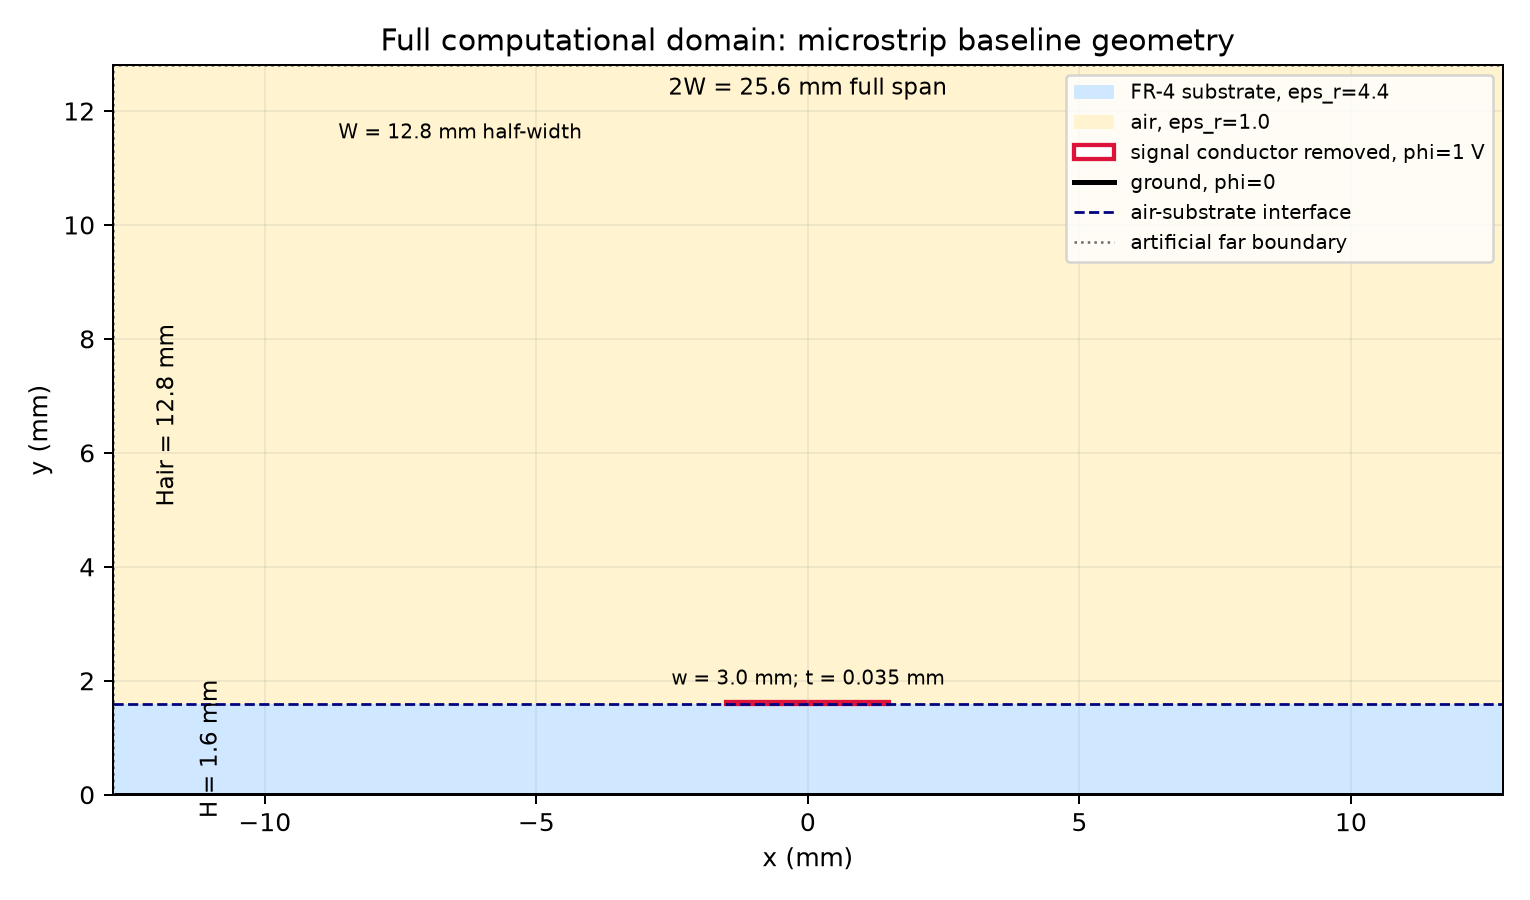
\includegraphics[width=\textwidth]{geometry_full_domain.png}
\caption{Final geometry convention. The domain half-width is $W$, so the full horizontal span is $2W$. The trace interior is removed from the field domain and the outer top and side boundaries are artificial truncation boundaries.}
\label{fig:geometry}
\end{figure}

\subsection{Governing equation and boundary conditions}
The field domain $\Omega$ is the computational rectangle with the conductor interior removed. The only PDE unknown is the electric potential $\phi(x,y)$, measured in volts. The material coefficient $\varepsilon(x,y)=\varepsilon_0\epsr(x,y)$ is prescribed in F/m, where $\varepsilon_0$ is the vacuum permittivity and $\epsr$ is the dimensionless relative permittivity. The gradient $\nabla\phi$ is the vector of spatial derivatives, and $d\Omega$ denotes area integration. The electrostatic energy model is described by Hiptmair~\cite[Sec.~1.2.2]{hiptmair2025}. For an admissible potential, the stored energy per unit length $W_e$ (J/m) is
\[
W_e(\phi)=\frac12\int_\Omega\varepsilon(x,y)|\nabla\phi|^2\,d\Omega.
\]
Stationarity of this energy with fixed conductor potentials gives the divergence-form equation below. The two materials have piecewise-constant permittivity: $4.4\varepsilon_0$ in the substrate and $\varepsilon_0$ in air. Hackbusch~\cite[Sec.~10.1]{hackbusch2017} explains why such positive discontinuous coefficients are naturally treated in a variational formulation, with separate integration over the material regions.

With no prescribed free volume charge, the potential $\phi$ satisfies
\begin{equation}
 -\nabla\cdot(\varepsilon \nabla \phi)=0
 \qquad \text{in }\Omega,
 \label{eq:pde}
\end{equation}
where $\nabla\cdot$ denotes divergence and $\varepsilon$ is the piecewise-constant material coefficient defined above. The essential boundary conditions are
\[
\phi=V_0 \quad \text{on the signal trace},\qquad
\phi=0 \quad \text{on the ground plane}.
\]
Let $\Gamma_{\rm far}$ denote the artificial top and side boundaries and let $n$ denote the outward unit normal on the field-domain boundary. They use the homogeneous Neumann condition
\[
\varepsilon \nabla \phi\cdot n=0.
\]
The electric field is $\mathbf E=-\nabla\phi$, measured in V/m, and the displacement field is $\mathbf D=\varepsilon\mathbf E$, measured in C/m$^2$. The zero Neumann condition therefore specifies zero normal displacement flux. This same far-boundary convention is used throughout the domain-truncation sequence. Across the air--substrate interface, the exact electrostatic interface conditions are continuity of potential and balance of normal displacement flux.

\section{Finite Element Formulation}
Let $\partial\Omega$ denote the entire field-domain boundary and $\Gamma_D$ the union of the trace and ground Dirichlet boundaries. The Sobolev space $H^1(\Omega)$ contains square-integrable functions with square-integrable first weak derivatives. The symbols $u$ and $v$ below denote admissible scalar functions and test functions, respectively; the sought physical potential remains $\phi$. The subscript $g$ refers to the prescribed boundary values. A lifting $g$ is any function in $H^1(\Omega)$ that matches the trace and ground voltages on $\Gamma_D$. The affine trial space is
\[
V_g=\{u\in H^1(\Omega):u=V_0 \text{ on the trace},\ u=0 \text{ on the ground}\},
\]
and the homogeneous test space is
\[
\mathcal V=\{v\in H^1(\Omega):v=0 \text{ on }\Gamma_D\}.
\]
Here $V_0$ denotes the prescribed trace voltage, while $\mathcal V$ denotes the homogeneous function space. Multiplying~\eqref{eq:pde} by $v\in\mathcal V$ and integrating by parts, with $ds$ denoting boundary arclength, gives
\[
\int_{\Omega} \varepsilon \nabla\phi\cdot\nabla v\,d\Omega
-\int_{\partial\Omega} \varepsilon \nabla\phi\cdot n\,v\,ds=0.
\]
The boundary term vanishes: $v=0$ on the Dirichlet boundaries, and the prescribed normal flux is zero on the remaining outer boundary. The weak problem is therefore:
\[
\text{find }\phi\in V_g\text{ such that }
\int_{\Omega}\varepsilon \nabla\phi\cdot\nabla v\,d\Omega=0
\quad\forall v\in\mathcal V.
\]

\subsection{Well-posedness and discrete stability}
The finite field domain is a connected bounded polygonal Lipschitz domain with the trace hole removed. The ground and trace together give $\Gamma_D$ positive boundary measure. The bilinear form $a(u,v)$ measures the permittivity-weighted gradient pairing. Writing $\|v\|_{L^2(\Omega)}=(\int_\Omega |v|^2\,d\Omega)^{1/2}$ for the square-integral norm, define
\[
a(u,v)=\int_\Omega\varepsilon\nabla u\cdot\nabla v\,d\Omega,
\qquad \varepsilon_0\le\varepsilon(x,y)\le4.4\varepsilon_0.
\]
Cauchy--Schwarz and the positive lower coefficient bound give
\begin{equation}
|a(u,v)|\le4.4\varepsilon_0\|\nabla u\|_{L^2}\|\nabla v\|_{L^2},
\qquad a(v,v)\ge\varepsilon_0\|\nabla v\|_{L^2}^2.
\label{eq:coercivity}
\end{equation}
For $v\in\mathcal V$, the Poincar\'e inequality
$\|v\|_{L^2}\le C_P\|\nabla v\|_{L^2}$ holds with a domain-dependent Poincar\'e constant $C_P$, because the Dirichlet boundary is nonempty with positive measure. The gradient seminorm is therefore a norm on $\mathcal V$, equivalent to its $H^1$ norm. The form $a$ is continuous and coercive even across the dielectric jump, since both material coefficients remain strictly positive.

Choose an $H^1$ lifting $g$ of the prescribed trace and ground values and write $\phi=g+u$. Here $u\in\mathcal V$ is the unknown homogeneous correction. Its load functional is $\ell(v)=-a(g,v)$, so the homogeneous problem is $a(u,v)=\ell(v)$ for all $v\in\mathcal V$. The load is bounded, so continuity and coercivity give existence and uniqueness by the Lax--Milgram theorem. In particular, the difference $\psi$ of two solutions satisfies $a(\psi,\psi)=0$, hence $\nabla\psi=0$; connectedness makes $\psi$ constant and its zero Dirichlet trace forces $\psi=0$. The Dirichlet constraints thus remove the constant nullspace that a pure-Neumann problem would have.

For a conforming triangular mesh $\mathcal T_h$, let $h$ denote a representative element diameter; $h_{\max}$ denotes the largest diameter in that mesh. The space $\mathcal V_h\subset\mathcal V$ consists of continuous functions affine on each triangle, with zero Dirichlet trace. Let $D$ be the prescribed-node index set, containing trace nodes $D_{\rm trace}$ and ground nodes $D_{\rm ground}$, and let $F$ be the complementary free-node set. If $K$ is the assembled stiffness matrix, whose entries have units F/m in this two-dimensional model, $K_{FF}$ is its free--free block. Let $z$ be a nonzero vector of free coefficients and $v_h\in\mathcal V_h$ its associated function. With $T$ denoting transpose, 
\[
z^T K_{FF}z=a(v_h,v_h)>0.
\]
Consequently, the reduced matrix is symmetric positive definite. Let $\delta\ell$ denote a perturbation of the load functional with unchanged Dirichlet data, and $\delta u_h$ the induced change in the discrete homogeneous solution. The dual space $\mathcal V^{\prime}$ contains continuous linear functionals on $\mathcal V$; its norm below uses the gradient norm. Testing the difference equation by $\delta u_h$ gives
\[
\|\nabla\delta u_h\|_{L^2}\le
\varepsilon_0^{-1}\|\delta\ell\|_{\mathcal V'},\qquad
\|\delta\ell\|_{\mathcal V'}=
\sup_{v\in\mathcal V\setminus\{0\}}
\frac{|\delta\ell(v)|}{\|\nabla v\|_{L^2}}.
\]
This estimate controls the solution in a function-space norm on the fixed domain. It does not bound the Euclidean matrix condition number independently of the mesh. Convergence speed is a separate issue, governed by solution regularity and mesh resolution. The measured energy-error exponent $p_E\simeq0.623$, defined as the slope of log energy error against log mesh size, is compatible with a stable problem whose corner/interface field is less regular than the smooth verification solution.

The well-posedness argument follows the standard variational theory for elliptic problems discussed by Hackbusch~\cite[Sec.~7.2]{hackbusch2017} and Quarteroni~\cite[Secs.~3.4 and 4.2]{quarteroni2017}. Their theory applies here because the permittivity stays strictly positive on both sides of the air--substrate interface. Quarteroni's Galerkin discussion also gives the positive-definite stiffness matrix on the homogeneous discrete test space.

\subsection{Assembly, solution and capacitance extraction}

The discrete space uses conforming triangular $P_1$ elements, as developed by Quarteroni~\cite[Sec.~4.5]{quarteroni2017} and Hiptmair~\cite[Sec.~2.4]{hiptmair2025}. Local element assembly and essential-boundary elimination follow the standard procedures described by Hiptmair~\cite[Secs.~2.7.4 and 2.7.6]{hiptmair2025}. Here $\phi_h$ is the finite-element approximation to $\phi$, $N_j$ is the dimensionless nodal basis function equal to one at node $j$ and zero at the other nodes, and $\Phi_j$ is the corresponding nodal potential in volts. Indices $i$ and $j$ run over mesh nodes. Writing
\[
\phi_h=\sum_j \Phi_j N_j,
\]
the stiffness matrix has entries
\[
K_{ij}=\int_{\Omega}\varepsilon \nabla N_i\cdot \nabla N_j\,d\Omega.
\]
Because $\varepsilon$ is discontinuous at the material interface, the integral is evaluated element by element using each triangle's material tag. In a conforming $H^1$ finite-element space, $\phi_h$ is continuous across the air--substrate interface. Elementwise integration of the discontinuous coefficient enforces interface flux balance in the global weak or distributional sense, without a separate Lagrange multiplier. The two elementwise $P_1$ normal-flux traces $\varepsilon\nabla\phi_h\cdot n$ can still differ pointwise along an interface edge.

The recorded environment uses scikit-fem 12.0.2 for mesh topology and the manufactured-solution basis, quadrature and assembly. For a triangle $K$ of area $|K|$ and material coefficient $\varepsilon_K$, let $K^K_{ij}$ denote its contribution to the global entry $K_{ij}$. For the microstrip solver, we evaluate the constant $P_1$ basis gradients explicitly and assemble $K^K_{ij}=\varepsilon_K|K|\nabla N_i\cdot\nabla N_j$ into a SciPy sparse matrix. This expression integrates the element stiffness exactly because the coefficient and gradients are constant on each material-conforming triangle. SciPy supplies the sparse direct solve. Our code defines the trace hole, material and boundary tags, refinement, capacitance extraction and validation. These model choices are tested separately from the library routines.

Writing $\Phi$ for the vector of nodal potentials, $\Phi_D$ contains prescribed values and $\Phi_F$ contains the unknown free values. Dirichlet elimination gives $K_{FF}\Phi_F=b_F$, where $b_F=-K_{FD}\Phi_D$ and $K_{FD}$ couples free and prescribed nodes. This sparse symmetric positive definite system is solved by a sparse direct solver. The full reaction vector is $r=K\Phi$; its Dirichlet entries represent charge reactions per unit length (C/m), while its free entries form the algebraic residual $r_F=K_{FF}\Phi_F-b_F$. For a vector, $\|\cdot\|_\infty$ denotes the largest absolute entry.

The capacitance is extracted in two ways. For the discrete field, the energy method defines $C_E$, the capacitance per unit length obtained from stored energy:
\[
W_e=\frac12\int_{\Omega}\varepsilon |\nabla \phi_h|^2\,d\Omega,\qquad
C_E=\frac{2W_e}{V_0^2}.
\]
The reaction-charge method sums the assembled Dirichlet reactions to obtain the trace charge per unit length $Q_{\rm trace}$ (C/m); $Q_{\rm ground}$ denotes the signed ground charge per unit length. The corresponding capacitance is $C_Q$ (F/m):
\[
C_Q=\frac{|Q_{\mathrm{trace}}|}{|V_0|}.
\]
The dimensionless extraction discrepancy is $\delta_{EQ}=|C_E-C_Q|/C_E$. Agreement between $C_E$ and $C_Q$ checks consistency of energy integration and reaction extraction. Geometry and boundary-tag tests are also required, since a shared modelling error could affect both quantities. Spatial accuracy is assessed through refinement.

\medskip
\begin{algorithm}[H]
\caption{Microstrip $P_1$ FEM solver}\label{alg:fem}
\begin{algorithmic}[1]
\Require Material-conforming mesh $\mathcal T_h$, geometry, $\varepsilon_K$ and voltage $V_0$
\State Generate the study mesh, or load the exact frozen mesh for a matched replay.
\State Verify the trace hole, interface, element regions and trace/ground/far boundary sets.
\State Set $D=D_{\rm trace}\cup D_{\rm ground}$, $F=\{\text{all nodes}\}\setminus D$.
\State Initialise $\Phi_D=V_0$ on the trace and $\Phi_D=0$ on ground; set $K=0$.
\For{each triangle $K_e\in\mathcal T_h$}
\State Compute $|K_e|$ and its three constant basis gradients.
\State Assemble $\varepsilon_{K_e}|K_e|\nabla N_i\cdot\nabla N_j$ into the sparse matrix.
\EndFor
\State Solve $K_{FF}\Phi_F=-K_{FD}\Phi_D$ by the sparse direct solver.
\State Evaluate $\nabla\phi_h$, $W_e$, $C_E=2W_e/V_0^2$ and reactions $r=K\Phi$.
\State Sum trace reactions to obtain $Q_{\rm trace}$ and $C_Q=|Q_{\rm trace}|/|V_0|$.
\State Check bounds, symmetry, residual, charge balance and $C_E/C_Q$ consistency.
\Ensure Potential, capacitances and diagnostics; failed checks disqualify interpretation.
\end{algorithmic}
\end{algorithm}
\medskip
In Algorithm~\ref{alg:fem}, the homogeneous Neumann edges add no load. Prescribed voltages enter the free system through $-K_{FD}\Phi_D$. Reactions must be recovered from the full assembled matrix, before its boundary rows are discarded. The implementation is in \path{code/fem_solver.py} and \path{code/capacitance.py}.

\section{Solver Verification and Baseline Checks}
\subsection{Manufactured-solution verification}
A known solution lets us measure discretisation error directly and compare the observed rates with smooth-solution estimates. This is the code-validation strategy discussed by Hiptmair~\cite[Sec.~3.8]{hiptmair2025}, with the expected finite-element energy and $L^2$ estimates given by Quarteroni~\cite[Sec.~4.5]{quarteroni2017}. Matching the rates supports the tested implementation; it does not by itself verify every feature of the microstrip model.

For this verification only, $u$ denotes a dimensionless exact solution, $u_h$ its finite-element approximation, and $f$ the manufactured source term; these symbols belong to the verification problem rather than the microstrip model. We use a unit square with zero Dirichlet data and exact solution
\[
u(x,y)=\sin(\pi x)\sin(\pi y).
\]
The manufactured forcing and boundary data are explicitly
\[
-\Delta u=f,\qquad f(x,y)=2\pi^2\sin(\pi x)\sin(\pi y),\qquad
u|_{\partial(0,1)^2}=0.
\]
Here $\Delta=\partial_{xx}+\partial_{yy}$ is the Laplacian and $e=u-u_h$ is the solution error. The named errors are $\|u-u_h\|_{L^2(\Omega)}$ and
$\|u-u_h\|_E=(\int_\Omega|\nabla(u-u_h)|^2\,d\Omega)^{1/2}$, with coefficient one for this verification problem. The expected smooth $P_1$ rates are two and one, respectively. The five consecutive meshes below contain the required $h,h/2,h/4,h/8$ protocol and one further level $h/16$. For refinement levels indexed by $i$, let $E_i$ be the selected $L^2$ or energy error and $h_i$ the corresponding maximum element diameter. The initial $h$ is the coarsest test scale. Pairwise observed orders $p_i$ are
$p_i=\log(E_{i-1}/E_i)/\log(h_{i-1}/h_i)$, where $\log$ denotes the natural logarithm.

\begin{figure}[H]
\centering
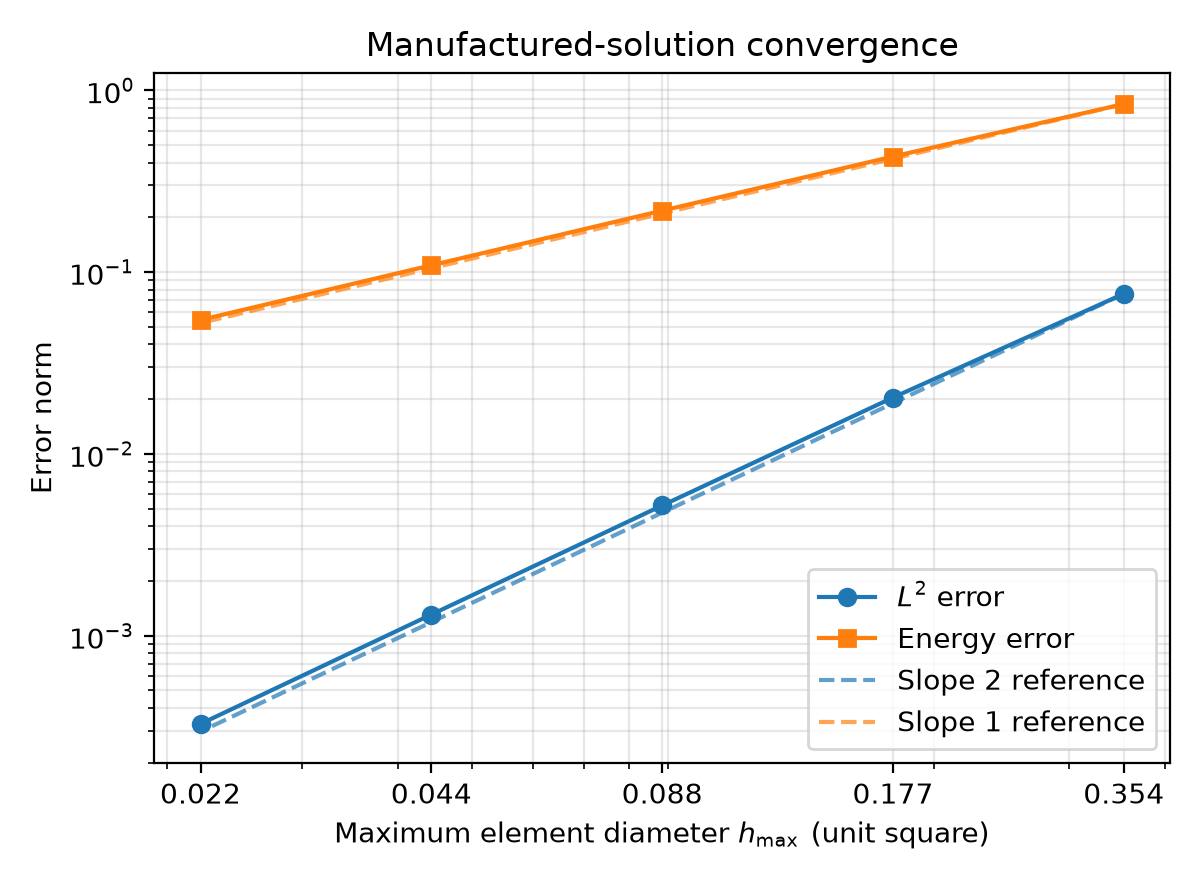
\includegraphics[width=0.82\textwidth]{mms_convergence_report.png}
\caption{Manufactured-solution convergence. The finest-step observed orders are approximately $2.00$ in $L^2$ and $1.00$ in the energy norm, as expected for smooth $P_1$ finite elements.}
\label{fig:mms}
\end{figure}

\begin{table}[H]
\centering
\small
\caption{Consecutive manufactured-solution refinements. $N_T$ is the triangle count and $r_F$ is the free-system algebraic residual. All five levels use a sparse direct solve; an iterative stopping tolerance is not applicable at any level.}
\label{tab:mms}
\begingroup
\setlength{\tabcolsep}{3pt}
\begin{tabular}{@{}lrrrrrrrr@{}}
\toprule
Level & $N_T$ & DOFs & $h_{\max}$ & $\|e\|_{L^2}$ & $\|e\|_E$ & $\|r_F\|_\infty$ & $p_{L^2}$ & $p_E$\\
\midrule
2 ($h$) & 32 & 25 & 0.35355 & $7.596\times10^{-2}$ & $8.397\times10^{-1}$ & $3.331\times10^{-16}$ & -- & --\\
3 ($h/2$) & 128 & 81 & 0.17678 & $2.041\times10^{-2}$ & $4.320\times10^{-1}$ & $5.551\times10^{-16}$ & 1.896 & 0.959\\
4 ($h/4$) & 512 & 289 & 0.08839 & $5.201\times10^{-3}$ & $2.176\times10^{-1}$ & $9.021\times10^{-16}$ & 1.972 & 0.989\\
5 ($h/8$) & 2048 & 1089 & 0.04419 & $1.307\times10^{-3}$ & $1.090\times10^{-1}$ & $1.457\times10^{-15}$ & 1.993 & 0.997\\
6 ($h/16$) & 8192 & 4225 & 0.02210 & $3.270\times10^{-4}$ & $5.451\times10^{-2}$ & $2.368\times10^{-15}$ & 1.998 & 0.999\\
\bottomrule
\end{tabular}

\endgroup
\end{table}

Least-squares fits of $\log E$ against $\log h_{\max}$ over the finest three levels (4--6) give
$p_{L^2}=\MMSLTwoFit$ and $p_E=\MMSEnergyFit$. The fitted and pairwise orders describe the same consecutive refinement sequence. The largest listed free residual is below $2.4\times10^{-15}$; the verification residual acceptance check is $\|r_F\|_\infty<10^{-10}$, not an iterative solver tolerance.

\subsection{Layered-interface analytic verification}
The layered problem from the Problem Pack checks the treatment of discontinuous coefficients. In this separate test, $a$ is the dimensionless material coefficient (not the bilinear form $a(u,v)$), $u_*$ is the prescribed analytic solution and $q_*$ its signed normal flux in the positive $x$ direction. On the dimensionless unit square, set $a=1$ for $x<1/2$ and $a=10$ for $x>1/2$, with $f=0$ and exact Dirichlet data on the entire boundary:
\[
u_*(x)=\begin{cases}20x/11,&x\le1/2,\\(2x+9)/11,&x\ge1/2.\end{cases}
\]
Both traces equal $10/11$ at the interface, while the gradients are $20/11$ and $2/11$. Thus the physical normal flux is $q_*=-a\partial_xu_*=-20/11$ on both sides. This checks the coefficient-weighted flux, rather than equality of the raw derivatives.

The test calls the production \texttt{assemble\_stiffness} routine with relative coefficients 1 and 10, then divides out the common $\varepsilon_0$ to obtain the dimensionless problem. Strong Dirichlet elimination is applied with the analytic boundary values. The fitted space contains the piecewise-affine exact solution, so its errors should be at round-off. Fitting a convergence slope to those errors would be uninformative.
\begin{table}[H]\centering\small
\caption{Layered verification using the actual production assembly. Here $N$ is the number of equal mesh intervals along each side of the unit square. Odd $N$ deliberately leaves the interface unresolved and assigns coefficients by element centroid; it is a negative control, not an acceptable reference method.}
\begin{tabular}{@{}lcrrr@{}}
\toprule
$N$ & Fitted? & DOFs & $\|u_h-u_*\|_\infty$ (nodes) & $\|q_h-q_*\|_{L^2}$\\
\midrule
4 & yes & 25 & 3.33e-16 & 3.18e-15\\
8 & yes & 81 & 8.88e-16 & 1.04e-14\\
16 & yes & 289 & 2.11e-15 & 3.86e-14\\
32 & yes & 1089 & 3.22e-15 & 9.15e-14\\
7 & no & 64 & 8.15e-02 & 1.07e+00\\
15 & no & 256 & 3.95e-02 & 5.80e-01\\
31 & no & 1024 & 1.94e-02 & 3.42e-01\\
\bottomrule
\end{tabular}
\label{tab:layered}
\end{table}
On fitted meshes the shared interface nodes enforce potential continuity, the maximum normal-flux jump is $2.28\times10^{-13}$, and the reduced matrices are symmetric with positive smallest eigenvalues. All solutions remain between zero and one. The unresolved control also has a small residual and a symmetric positive matrix, yet has much larger solution and flux errors. This control shows that solving the discrete equations accurately does not establish that the interface was represented correctly.
\begin{figure}[H]\centering
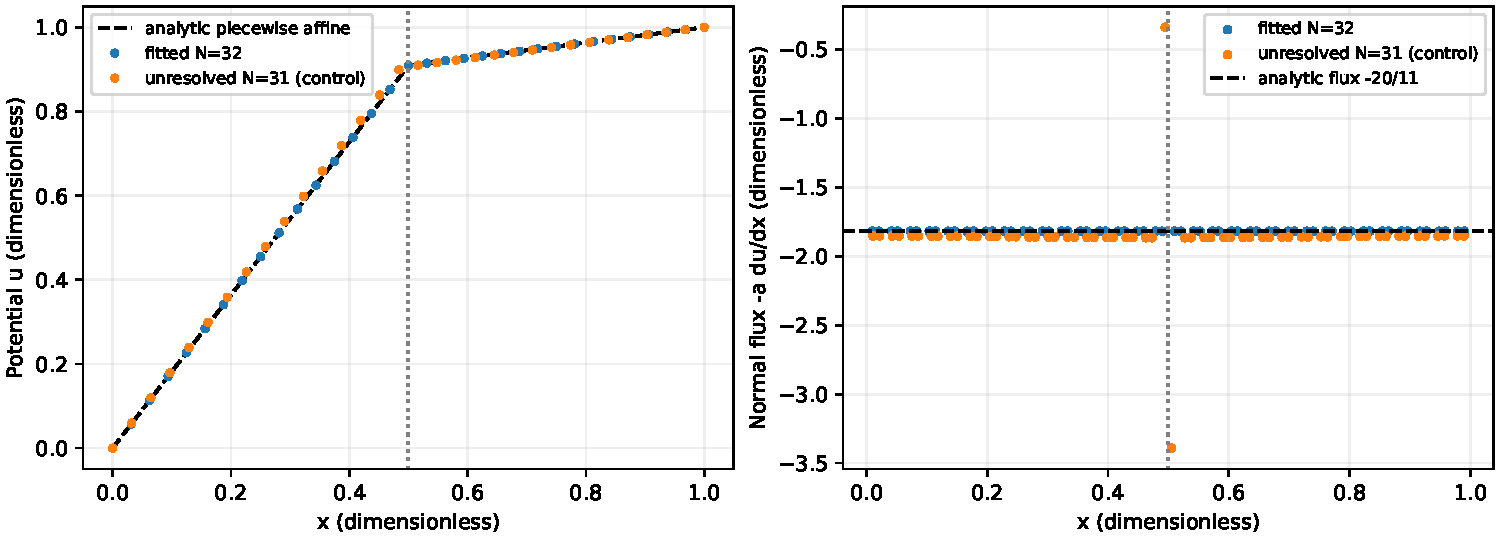
\includegraphics[width=\textwidth]{ae_revision/layered_interface_verification.pdf}
\caption{Analytic potential and normal flux across the two materials. The fitted solution reproduces both; the unresolved centroid-tag control shows why accurate interface representation must be checked separately.}
\label{fig:layered}
\end{figure}

\subsection{Baseline microstrip sanity checks}
Nodal reflection symmetry compares the potential vector with its values at $(-x,y)$ using the relative Euclidean norm. Matrix symmetry uses the Frobenius norm of $K_{FF}-K_{FF}^T$ divided by that of $K_{FF}$. The charge-balance defect is the absolute sum of the signed trace and ground reactions, normalised by the largest of their magnitudes and $C_E|V_0|$. The representative baseline solve passed the expected physical and algebraic checks. The potential remained in the interval $[0,1]$, the symmetry error about $x=0$ was near round-off, the reduced matrix symmetry error was zero to numerical precision, and the residual was negligible. The energy and reaction capacitances agreed to within $2.54\times10^{-15}$ relative difference.

\paragraph{Linear solver and algebraic-error control.}
The sparse symmetric positive definite free system is small enough for a direct solve at the tested sizes. This avoids choosing an iterative stopping tolerance. To assess algebraic error, we consider conditioning as well as the residual. The physical condition estimate is the ratio of the largest to smallest eigenvalue of $K_{FF}$. For diagonal scaling, let $D_K$ be the diagonal matrix formed from the positive diagonal of $K_{FF}$; the scaled diagnostic is the corresponding eigenvalue ratio of $D_K^{-1/2}K_{FF}D_K^{-1/2}$. For the representative baseline solve, the estimated physical reduced-system condition number was $1.7922363\times10^5$, while the diagonal-scaled diagnostic was $1.4249857\times10^4$. The free residual infinity norm was $3.101927\times10^{-25}$. The scaled estimate belongs to the scaled matrix, not the physical one. Together with the small backward residual, these condition diagnostics indicate algebraic error well below the observed finite-element discretisation effects.

\begin{table}[H]
\centering
\small
\caption{Representative baseline checks on the $8H$ microstrip domain.}
\label{tab:baseline}
\begin{tabular}{@{}ll@{}}
\toprule
Diagnostic & Value\\
\midrule
Potential range & $[0,1]$\\
Symmetry relative error & $3.244\times10^{-14}$\\
Reduced-matrix symmetry error & $0$\\
Smallest eigenvalue estimate & $5.918\times10^{-15}$\\
Largest eigenvalue estimate & $1.060677\times10^{-9}$\\
Condition estimate & $1.7922363\times10^5$\\
Diagonal-scaled condition diagnostic & $1.4249857\times10^4$\\
Free residual infinity norm & $3.101927\times10^{-25}$\\
$C_E$ and $C_Q$ diagnostic difference & $2.536\times10^{-15}$\\
Charge-balance defect & $6.973\times10^{-15}$\\
\bottomrule
\end{tabular}
\end{table}

\begin{figure}[H]
\centering
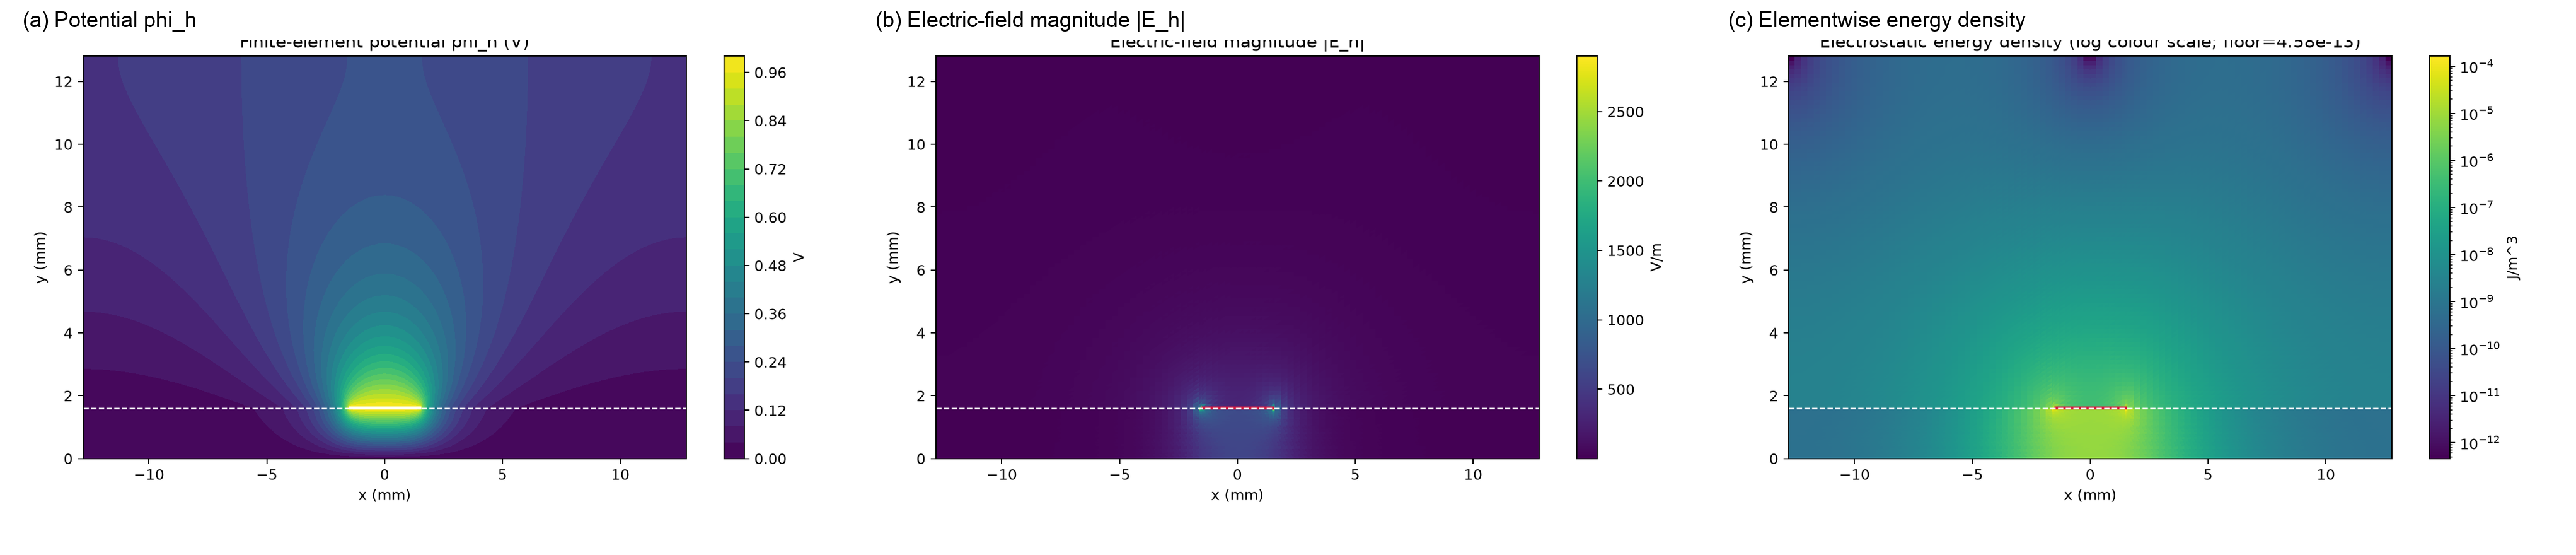
\includegraphics[width=\textwidth]{baseline_field_diagnostics.png}
\caption{Baseline field diagnostics: (a) finite-element potential $\phi_h$, (b) electric-field magnitude $|\mathbf E_h|$ with $\mathbf E_h=-\nabla\phi_h$, and (c) elementwise electrostatic energy density $\tfrac12\varepsilon|\mathbf E_h|^2$ (J/m$^3$), shown with a logarithmic colour scale for visibility. The potential respects the imposed Dirichlet values, while the field and energy density concentrate near the trace corners. These plots are diagnostic visualisations, not error norms.}
\label{fig:baseline-fields}
\end{figure}

\section{Domain Truncation}
We approximate the unbounded air region by a finite rectangle. To isolate the effect of this truncation, we used the sequence $(W/H,H_{\mathrm{air}}/H)=(3,3),(5,5),(8,8),(12,12)$ while preserving the near-trace mesh. The $12H$ result was used only as a tested finite-domain reference, not as the exact infinite-domain solution.

\begin{figure}[H]
\centering
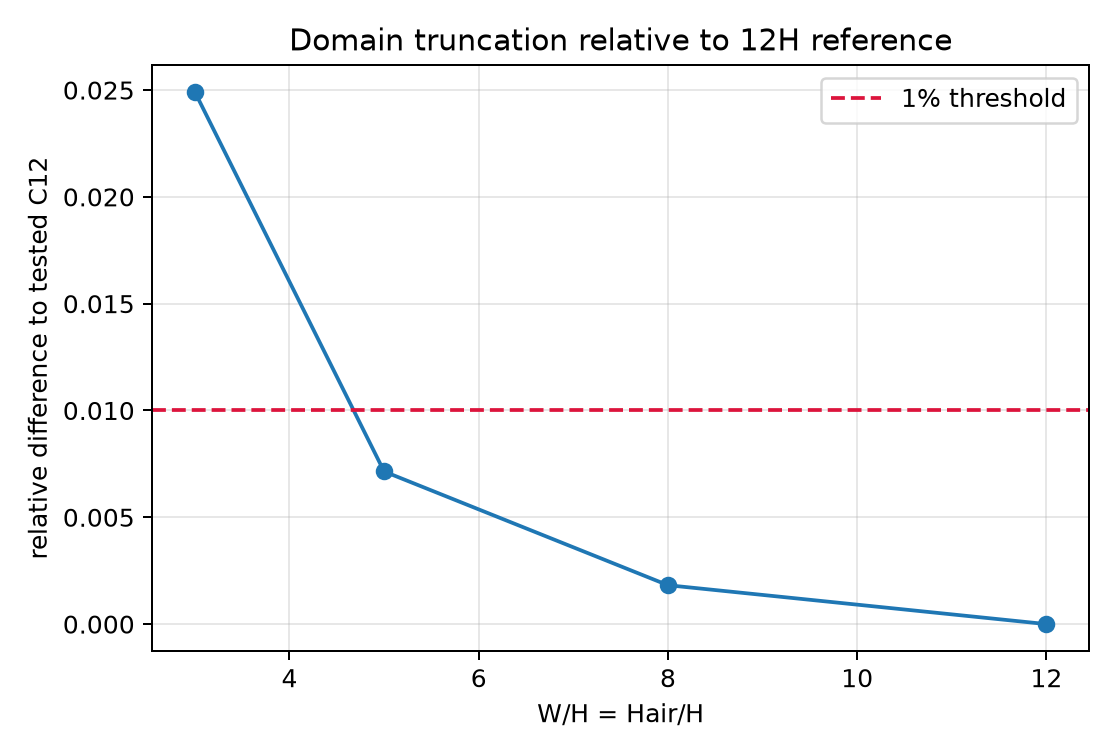
\includegraphics[width=0.82\textwidth]{domain_truncation.png}
\caption{Domain-truncation study. Differences are relative to the tested $12H$ finite-domain reference. The horizontal line marks the one-percent threshold.}
\label{fig:domain}
\end{figure}

\begin{table}[H]
\centering
\small
\caption{Production domain-truncation results.}
\label{tab:domain}
\begin{tabular}{@{}rrrrr@{}}
\toprule
$W/H=H_{\mathrm{air}}/H$ & Elements & DOFs & $C_E$ (pF/m) & Difference from $12H$\\
\midrule
3 & 11868 & 6121 & 118.839 & $2.491\%$\\
5 & 16988 & 8711 & 121.004 & $0.714\%$\\
8 & 26168 & 13346 & 121.653 & $0.182\%$\\
12 & 41208 & 20926 & 121.875 & reference\\
\bottomrule
\end{tabular}
\end{table}

In this domain study, $C_{12,R0}$ denotes the $12H$ production-mesh capacitance and $C_{12,R1}$ the finer repeat; $R0$ and $R1$ here are domain-resolution labels. The largest-domain mesh-adequacy check repeated the $12H$ case with a finer near-field resolution. The production value was
$C_{12,R0}=1.2187452011154754\times10^{-10}\,\mathrm{F/m}$, while the refined repeat gave
$C_{12,R1}=1.2183061087416544\times10^{-10}\,\mathrm{F/m}$. The resulting mesh sensitivity was $3.604122\times10^{-4}$, or about $0.0360\%$. This is smaller than the $8H$--to--$12H$ production difference of about $0.182\%$, supporting the domain choice without attributing the production difference mainly to near-field mesh resolution. Neither $12H$ value is treated as the exact infinite-domain capacitance.

The production $8H$ value in Table~\ref{tab:domain}, $121.653\,\mathrm{pF/m}$, and the final M7 value, $120.620\,\mathrm{pF/m}$, use different mesh families and resolutions. Their difference includes mesh-resolution effects and cannot be assigned solely to truncation. The $0.182\%$ indicator compares matched-core production-domain meshes; it is not a measured truncation error, or an upper bound, for M7. The finer $12H$ repeat strengthens the original domain decision but does not replace a matched-M7-resolution $8H/12H$ study, which has not been performed.

The smallest tested domain below one percent was $5H$. The later studies use the $8H$ domain because its tested difference from $12H$ was only about $0.182\%$ while remaining substantially cheaper than the largest domain. This is a finite-domain sensitivity indicator rather than a rigorous infinite-domain error bound.

\section{Mesh Convergence and Corner Singularity}
\subsection{Corner-field behaviour}
Finite-element error estimates depend on solution regularity as well as the approximation space. Hackbusch~\cite[Secs.~8.5 and 9.1]{hackbusch2017} and Hiptmair~\cite[Sec.~3.4]{hiptmair2025} discuss this dependence and the effect of nonsmooth domains. This theory explains the dependence on smoothness, but does not predict our measured value of $0.623$.

The field is singular near the conductor corners. At the lower corners, the conductor boundary also meets the air--substrate interface. A mesh-dependent peak field that increases under refinement is therefore consistent with singular behaviour; it is not itself an accuracy norm.

\begin{figure}[H]
\centering
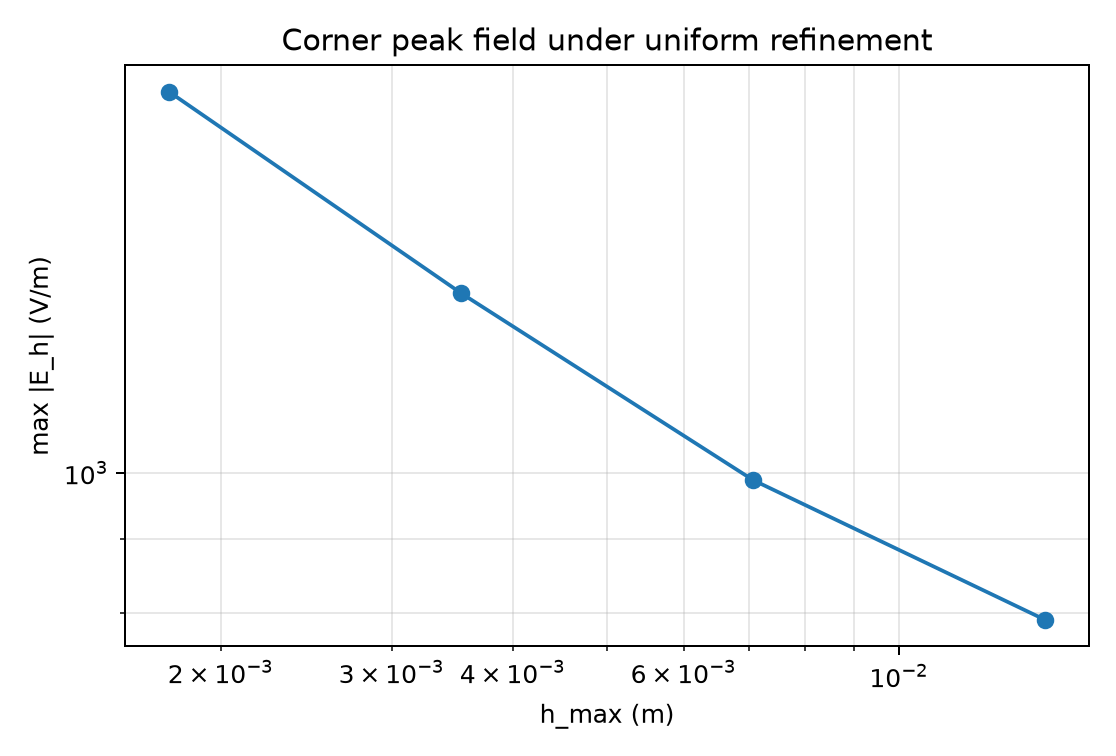
\includegraphics[width=0.82\textwidth]{corner_max_field_vs_h.png}
\caption{Maximum computed electric-field magnitude under uniform refinement. The increasing peak is consistent with stronger resolution of the trace-corner field.}
\label{fig:corner}
\end{figure}

\subsection{Uniform energy-norm convergence}
In the uniform hierarchy, $M_j$ denotes the base mesh M0 after $j$ global refinements, each approximately halving $h_{\max}$. The reference-mesh labels in this section are $R0=M4$, $R1=M5$ and $R2=M6$, distinct from the domain-resolution labels used above. Uniform convergence was measured against $R2=M6$. Let $\phi_{\rm ref}$ be the reference potential and $e=\phi_{\rm ref}-\phi_h$ the field error. The subscript $E$ denotes the permittivity-weighted energy norm:
\[
\|e\|_E^2=\int_{\Omega}\varepsilon |\nabla(\phi_{\mathrm{ref}}-\phi_h)|^2\,d\Omega.
\]
The dimensionless relative energy error $E_{\mathrm{rel}}^{\mathrm{ref}}$ used in the figures and tables is
\begin{equation}
E_{\mathrm{rel}}^{\mathrm{ref}}=
\frac{\|\phi_{\mathrm{ref}}-\phi_h\|_E}{\|\phi_{\mathrm{ref}}\|_E},\qquad
\|\phi_{\mathrm{ref}}\|_E^2=\int_\Omega\varepsilon|\nabla\phi_{\mathrm{ref}}|^2\,d\Omega.
\label{eq:relative-energy}
\end{equation}
When the reference changes, both numerator and denominator use that same reference; this dimensionless ratio is not a relative capacitance difference.
Coefficient vectors on different meshes were never directly subtracted. Instead, the coarse $P_1$ gradient was evaluated on the reference mesh elements and the error was integrated on the reference grid.

\begin{figure}[H]
\centering
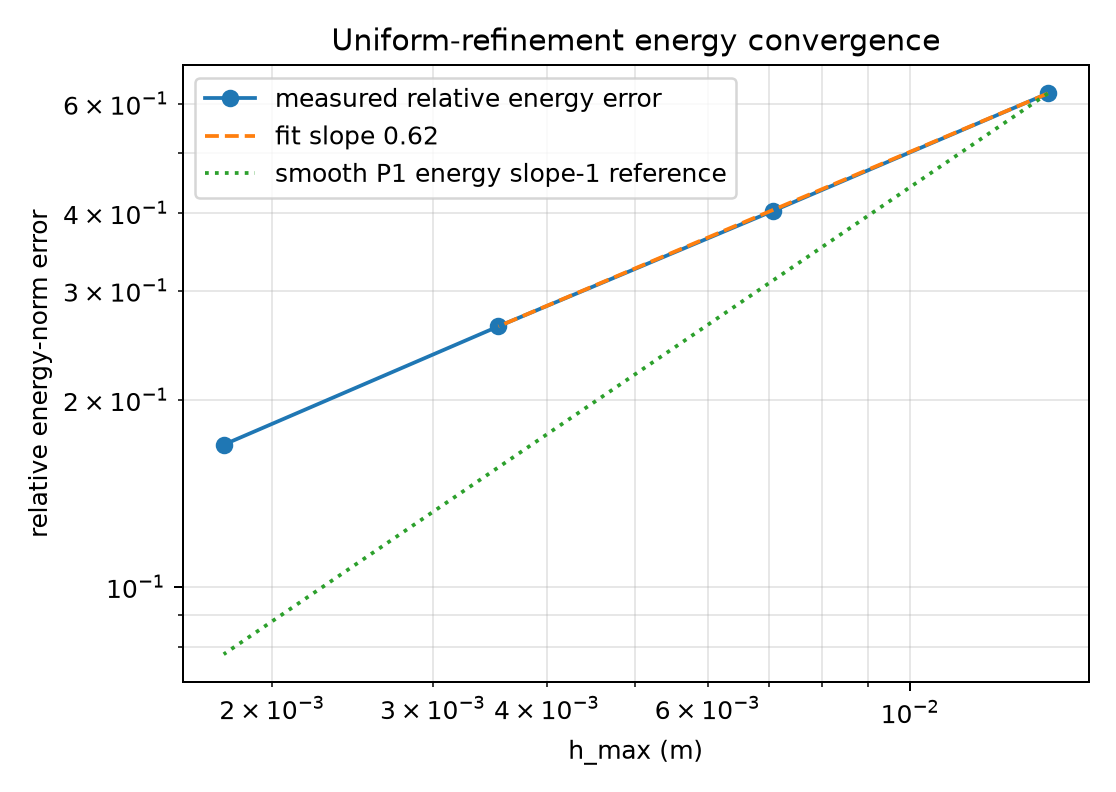
\includegraphics[width=0.82\textwidth]{uniform_energy_convergence.png}
\caption{Uniform-refinement energy-norm convergence. The fitted slope over M0--M2 is about $0.623$, below the smooth $P_1$ energy slope of one.}
\label{fig:uniform}
\end{figure}

\begin{table}[H]
\centering
\small
\caption{Uniform energy-error convergence against the accepted $R2=M6$ reference.}
\label{tab:uniform}
\begin{tabular}{@{}rrrrr@{}}
\toprule
Mesh & DOFs & $h_{\max}$ (m) & Relative energy error & $C_E$ (pF/m)\\
\midrule
M0 & 35 & $1.415\times10^{-2}$ & 0.6230 & 167.703\\
M1 & 114 & $7.077\times10^{-3}$ & 0.4030 & 140.432\\
M2 & 404 & $3.538\times10^{-3}$ & 0.2627 & 129.144\\
M3 & 1512 & $1.769\times10^{-3}$ & 0.1694 & 124.273\\
\bottomrule
\end{tabular}
\end{table}

\begin{table}[H]
\centering
\small
\caption{Reference stability in the M0--M2 fit window. R0=M4, R1=M5 and R2=M6. The last column is $|E_{\rm rel}^{R2}-E_{\rm rel}^{R1}|/|E_{\rm rel}^{R2}|$; each relative error is normalised as in~\eqref{eq:relative-energy}.}
\label{tab:reference-stability}
\begin{tabular}{@{}lrrrr@{}}
\toprule
Mesh & $E_{\rm rel}^{R0}$ & $E_{\rm rel}^{R1}$ & $E_{\rm rel}^{R2}$ & $R1\to R2$ change\\
\midrule
M0 & 0.610595 & 0.619193 & 0.623045 & $0.618\%$\\
M1 & 0.386757 & 0.398039 & 0.403041 & $1.241\%$\\
M2 & 0.239121 & 0.255580 & 0.262690 & $2.707\%$\\
\bottomrule
\end{tabular}

\end{table}

The accepted fitted slope is $0.623$ over M0--M2. The R1-to-R2 changes in Table~\ref{tab:reference-stability} range from $0.618\%$ to $2.707\%$; changing the reference changes the fitted slope from $\RefSlopeROne$ to $\RefSlopeRTwo$. Both fits remain sublinear after reference refinement. The sensitivity is finite and is not treated as zero or as a rigorous negligible-error bound. M3 is excluded from the fit because its R1-to-R2 error sensitivity is larger ($6.384\%$). The reduced rate is consistent with conductor-corner and material-interface regularity loss.

\paragraph{Fit-window robustness.}
Table~\ref{tab:fit-robustness} compares different references and fit windows; all data are retained. With R2, the adjacent M0--M1 and M1--M2 slopes are $0.6284$ and $0.6176$; adding M3 gives $0.6255$, but M3 has the larger disclosed reference sensitivity. The three-point $0.623$ fit describes the tested coarse range; it does not identify a precise singular exponent or establish an asymptotic rate. R0 changes that same fit to $0.6762$, showing why the over-refined reference matters.
\begin{table}[H]\centering\small
\caption{Existing-data sensitivity of the uniform energy fit. The accepted M0--M2/R2 fit is unchanged; the other rows test its interpretation.}
\begin{tabular}{@{}llrr@{}}
\toprule
Window & Reference & Points & Fitted $h$ slope\\
\midrule
M0-M2 & R0 & 3 & 0.676239\\
M0-M2 & R1 & 3 & 0.638307\\
M0-M2 & R2 & 3 & 0.622987\\
M0-M3 & R2 & 4 & 0.625473\\
\bottomrule
\end{tabular}
\label{tab:fit-robustness}
\end{table}

\section{Historical Graded Refinement and Integration Limitation}
\label{sec:historical-graded}
We tested whether concentrating coordinate-line refinement near the four trace corners could improve efficiency, with additional emphasis on the lower conductor/material-junction corners. The method remained symmetric about $x=0$ and used the same physical model as the uniform sequence.

\paragraph{Reproducible grading rule.}
Let $B_x$ and $B_y$ be the shared base sets of horizontal and vertical coordinates. In units of $H$, they are
\[
B_x/H=(-8,-2,-0.9375,0,0.9375,2,8),\qquad
B_y/H=(0,1,1.021875,1.5,8).
\]
For a coordinate set $B$ and a nonnegative integer depth $k$, let $D_k(B)$ bisect every interval exactly $k$ times (ratio $1/2$). The integer parameters $(b,u,\ell)$ specify background, upper-corner and lower-junction refinement depths, respectively; $u$ here is a grading parameter rather than a potential. The labels G0--G4 identify the five resulting graded meshes. For these parameters, retain the background coordinates $D_b(B_x)$ and $D_b(B_y)$. Add coordinates from $D_\ell(B_x)$ within $0.45H$ of either $x=\pm w/2$ and from $D_\ell(B_y)$ within $0.45H$ of $y=H$. Add coordinates from $D_u(B_x)$ within $0.30H$ of either $x=\pm w/2$ and from $D_u(B_y)$ within $0.30H$ of $y=H+t$. Take sorted unions, snap to the M6 coordinate set at $10^{-15}\,\mathrm{m}$ precision, form the Cartesian grid, and split each retained rectangle along its bottom-left/top-right diagonal; remove the trace interior. These are axis-aligned bands, not circular element-distance zones: adding a coordinate line also spends resolution away from a corner.

\begin{table}[H]
\centering
\small
\caption{Deterministic G-level parameters read from the experiment CSV. $b$ is the background depth, $u$ the upper-corner depth, and $\ell$ the lower-junction depth. The lower corners receive one extra depth for G0--G3; G4 uses depth five for both, with the larger lower-corner band retained.}
\label{tab:grading-rule}
\begin{tabular}{@{}lrrrrr@{}}
\toprule
Mesh & $b$ & $u$ & $\ell$ & DOFs & Min. corner size (m)\\
\midrule
G0 & 0 & 1 & 2 & 123 & $4.210\times10^{-4}$\\
G1 & 1 & 2 & 3 & 537 & $2.105\times10^{-4}$\\
G2 & 1 & 3 & 4 & 1422 & $1.052\times10^{-4}$\\
G3 & 2 & 4 & 5 & 5306 & $5.262\times10^{-5}$\\
G4 & 3 & 5 & 5 & 7068 & $5.262\times10^{-5}$\\
\bottomrule
\end{tabular}

\end{table}

\begin{figure}[H]
\centering
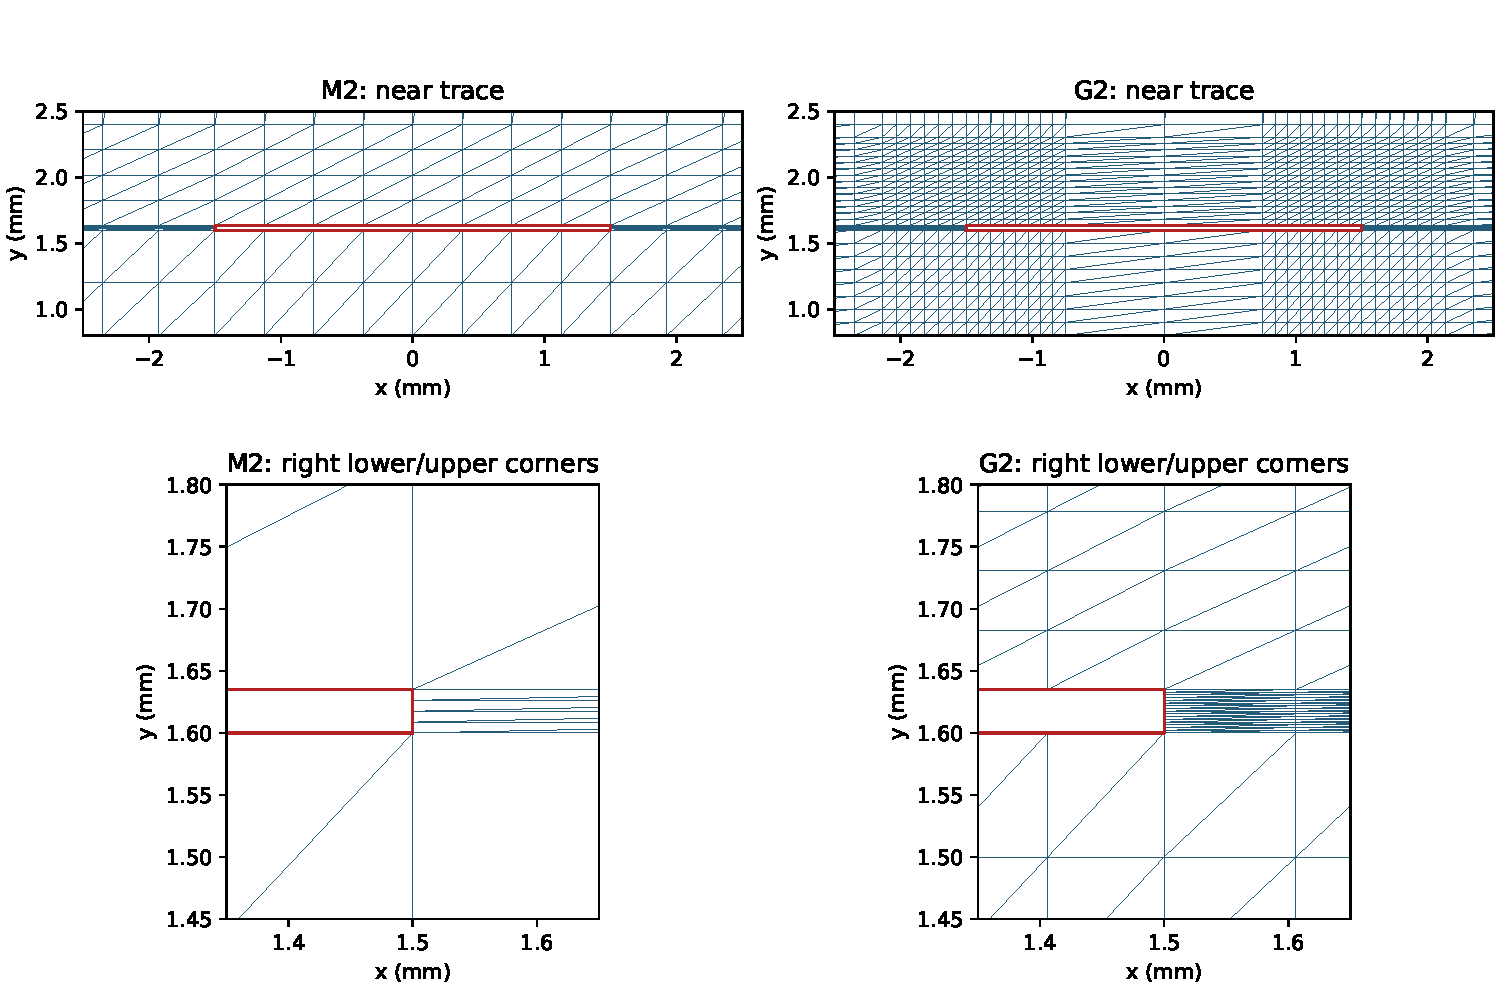
\includegraphics[width=\textwidth]{ae_revision/uniform_graded_corner_mesh.pdf}
\caption{Saved uniform M2 and graded G2 meshes, with an additional right-corner enlargement. These are geometry views, not a matched-DOF efficiency claim; the three-method overlay comparison below uses the measured work metrics.}
\label{fig:meshcompare}
\end{figure}

\begin{figure}[H]
\centering
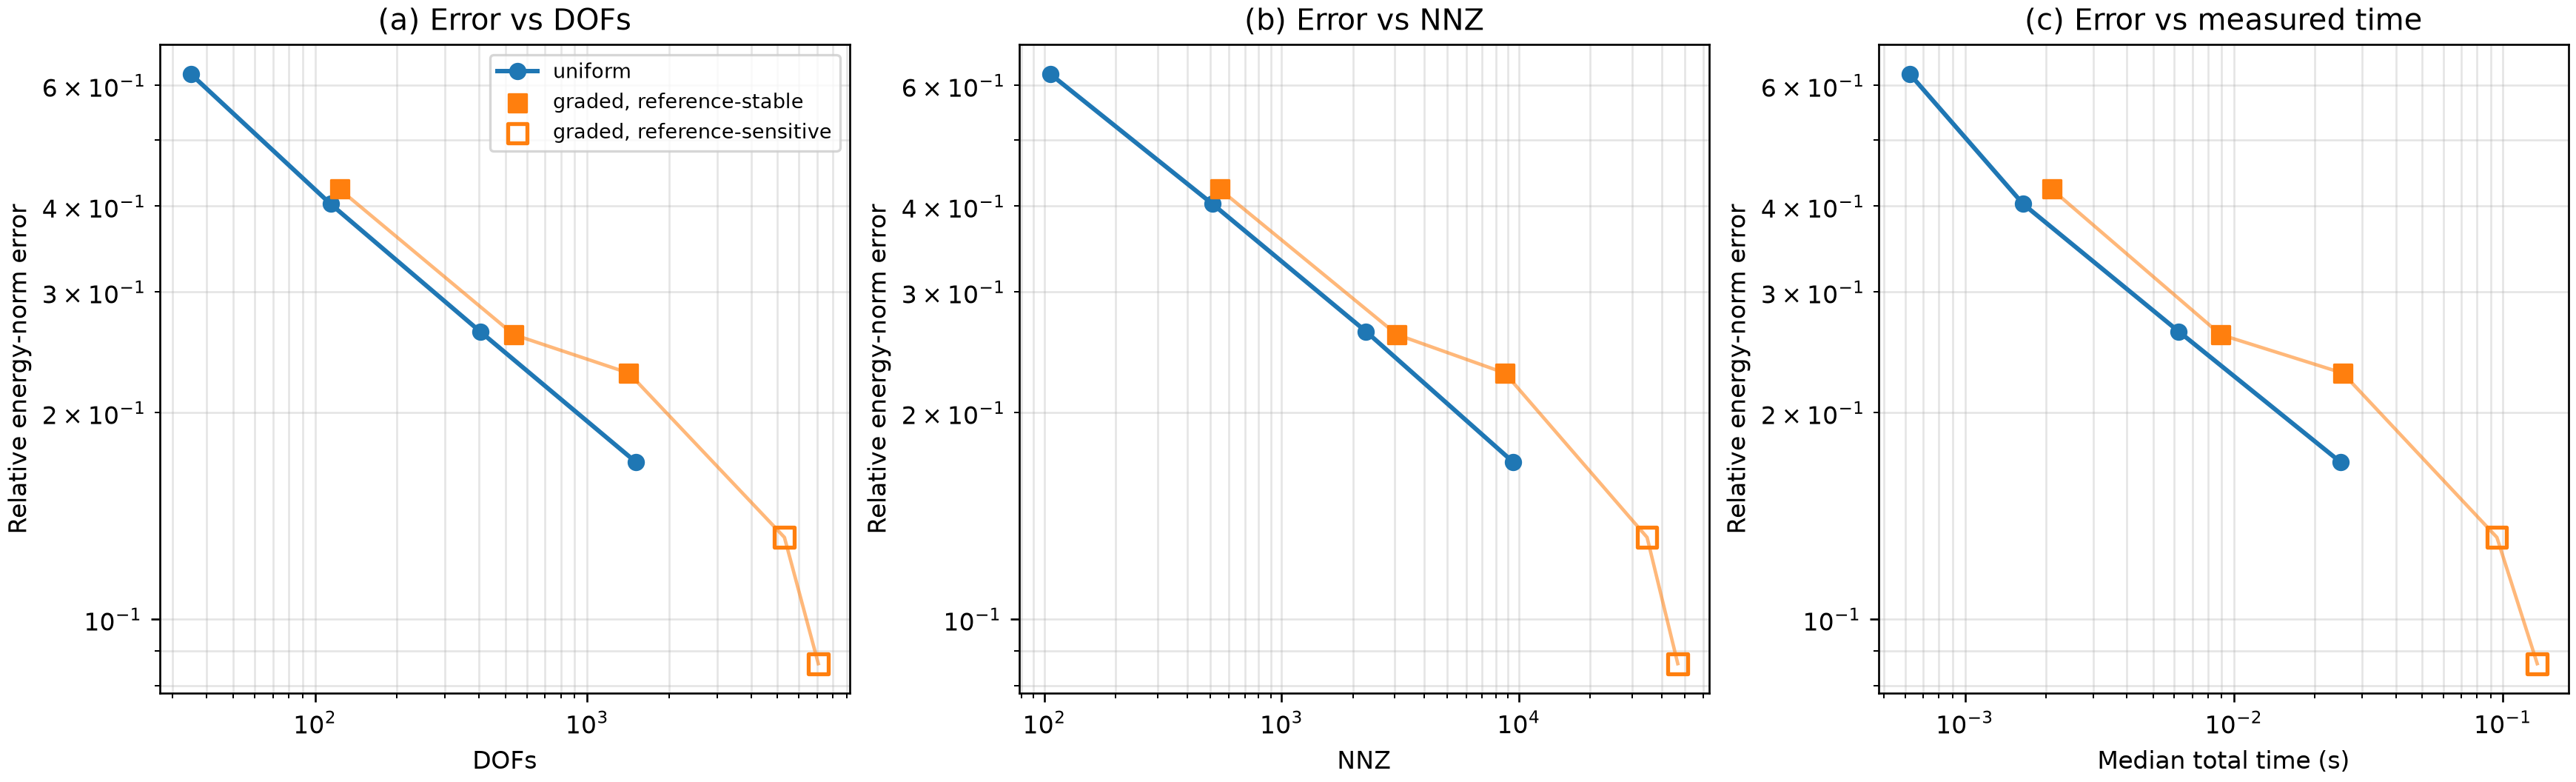
\includegraphics[width=\textwidth]{graded_cost_metrics.png}
\caption{Historical exploratory estimates against (a) DOFs, (b) NNZ and (c) median time, retained unchanged. Filled orange squares pass the original reference-sensitivity check, but that check does not validate the cross-mesh integration. These curves do not support precise efficiency ratios; Figure~\ref{fig:adaptive-work} supplies the validated exact-overlay comparison.}
\label{fig:graded-cost}
\end{figure}

The saved estimates initially suggested no clear cost--accuracy advantage for grading, including at targets $0.40$ and $0.30$, despite finer corner resolution. The later crossing check showed that the error integration was not always valid. We therefore retain these curves as exploratory results.

\paragraph{Why the comparison was repeated.}
The coordinate-subset assumption did not ensure nested triangles. For G2, $21440$ of the $180224$ reference triangles cross a coarse diagonal, covering about $4.55\%$ of field-domain area. This is not an error bound. We kept the original results and the safety guard, then repeated the comparison with triangle-overlay integration in Section~\ref{sec:residual-adaptive}. Appendix~A, case audit~3 records the geometric test, replacement method and exact evidence locations.

As discussed by Hiptmair~\cite[Sec.~3.5]{hiptmair2025}, numerical quadrature can introduce additional errors into a finite-element calculation. In our original graded-mesh comparison, some reference triangles crossed coarse-element boundaries where the gradient was discontinuous. We therefore replaced the centroid-based error integration with triangle-overlay integration before making quantitative efficiency comparisons. Here the approximation affected error-norm post-processing, rather than the production stiffness assembly. The crossed-triangle count, $4.55\%$ area fraction and corrected results are our own measurements, not conclusions taken from the text.

This result motivated residual-driven marking, in which the computed flux imbalance determines the elements to refine instead of prescribed corner bands.

\section{Residual-Based Adaptive Refinement}
\label{sec:residual-adaptive}
\subsection{Motivation and controlled setup}
The reduced uniform energy rate, $p_E\simeq0.623$, and the absence of a measured advantage for the prescribed coordinate-line grading motivated a solution-driven extension. The hypothesis was recorded before the experiments in \texttt{logs/PRE\_ADAPTIVE\_HYPOTHESIS.md}. No advantage was assumed. The $8H$ domain, trace hole, material coefficient, homogeneous-Neumann far boundary, $P_1$ formulation and sparse direct solver were held fixed. No new all-air problem was solved, and the final M7 engineering values were not changed.

The historical M2 coordinates are left--right symmetric, but its identically oriented cell diagonals are not. To avoid confusing mesh-orientation asymmetry with adaptivity, the primary initial mesh uses a conforming, mirror-invariant subdivision of M1. All edge midpoints are inserted; each right triangle is divided into four nonobtuse triangles, giving exactly the M2 coordinates, $704$ elements and $404$ DOFs. We call this \emph{M1-S (M2-resolution)}, not the unchanged M2 triangulation. An eight-cycle M0-S companion path brackets the $0.40$ and $0.30$ error targets, since the primary initial error is already below $0.30$.

An earlier diagonal-only symmetry completion was rejected: its very coarse M0 companion produced minimum potentials down to about $-0.030$ V. All its points and timings remain in a separate failed-attempt directory and are excluded from the conclusions. The correction was made to satisfy potential bounds, not to optimise efficiency; the indicator and marking parameter were unchanged.

\subsection{Flux-jump indicator and marking}
For $f=0$, constant elementwise $\epsilon$ and affine $\phi_h|_K$, the interior volume residual vanishes. For an interior edge, choose one unit normal $n_e$ and define
\[
J_e=(\epsilon\nabla\phi_h|_{K^+}-\epsilon\nabla\phi_h|_{K^-})\cdot n_e.
\]
The same normal is used on both sides, including material-interface edges. With $h_e$ equal to edge length, the implemented indicator is
\begin{equation}
\eta_K^2=\frac12\sum_{e\subset\partial K\cap\mathcal E_{\rm int}}
h_e\|J_e\|_{L^2(e)}^2+
\sum_{e\subset\partial K\cap\Gamma_{\rm far}}
h_e\|\epsilon\nabla\phi_h\cdot n\|_{L^2(e)}^2,
\qquad \eta=\left(\sum_K\eta_K^2\right)^{1/2}.
\end{equation}
Since these traces are constant, each term is evaluated exactly as $h_e^2J_e^2$ (or its boundary counterpart). Trace and ground Dirichlet edges contribute no natural-boundary residual. This is a \emph{residual-based refinement indicator}, not a guaranteed error bound.

At every step, deterministic D\"orfler marking chooses the smallest descending-indicator prefix containing at least $\theta=0.5$ of $\sum_K\eta_K^2$. The reflected triangles are added for symmetry. All edges of marked triangles are split; any triangle with two split edges has its third edge split as well. This conformity closure gives unambiguous red/four-child and green/two-child subdivisions. Minimal marks, symmetry-added marks and all actually refined parents are recorded separately. No corner-distance rule selects elements.

\subsection{Reference error and adaptive mesh behaviour}
The principal and sensitivity references are M6 and the frozen M7 dielectric solution. For $R\in\{M6,M7\}$,
\[
\|e_R\|_E=\left(\int_\Omega\epsilon|\nabla(\phi_R-\phi_h)|^2\,d\Omega\right)^{1/2},\quad
E_{{\rm rel},R}=\frac{\|e_R\|_E}{\|\phi_R\|_E},\quad
S_{\rm ref}=\frac{|\|e_{M7}\|_E-\|e_{M6}\|_E|}{\|e_{M7}\|_E}.
\]
All three methods are newly compared using $E_{{\rm rel},M6}$ and the same exact triangle-overlay integration. Contained reference triangles use constant gradients directly; crossed triangles are intersected geometrically and integrated by overlap area. Coefficient vectors on different meshes are never subtracted. This also resolves the integration issue identified in Section~7 for the \emph{new} comparison, without changing its historical Figure~8 or raw tables. The maximum relative overlay area-coverage defect was below $2\times10^{-12}$. Formal comparisons require $S_{\rm ref}<3\%$; other points remain visible with open markers.

\begin{table}[H]
\centering\small
\caption{Primary residual-adaptive sequence. Every point meets the predeclared reference-sensitivity criterion. Full-precision capacitances, marks, sanity checks and timing samples are retained in the extension CSVs.}
\begin{tabular}{@{}lrrrrr@{}}
\toprule
Cycle & Elements & DOFs & NNZ & $E_{\rm rel}$ & $S_{\rm ref}$ (\%)\\
\midrule
A0 & 704 & 404 & 2265 & 0.2637 & 0.847\\
A1 & 758 & 432 & 2439 & 0.2279 & 1.123\\
A2 & 898 & 504 & 2891 & 0.2056 & 1.325\\
A3 & 1218 & 666 & 3973 & 0.1789 & 1.610\\
A4 & 1650 & 890 & 5381 & 0.1670 & 1.600\\
A5 & 2270 & 1206 & 7469 & 0.1553 & 0.941\\
A6 & 3040 & 1602 & 10019 & 0.1434 & 0.297\\
A7 & 4008 & 2088 & 13345 & 0.1354 & 0.412\\
\bottomrule
\end{tabular}

\label{tab:adaptive-sequence}
\end{table}

\begin{figure}[H]
\centering
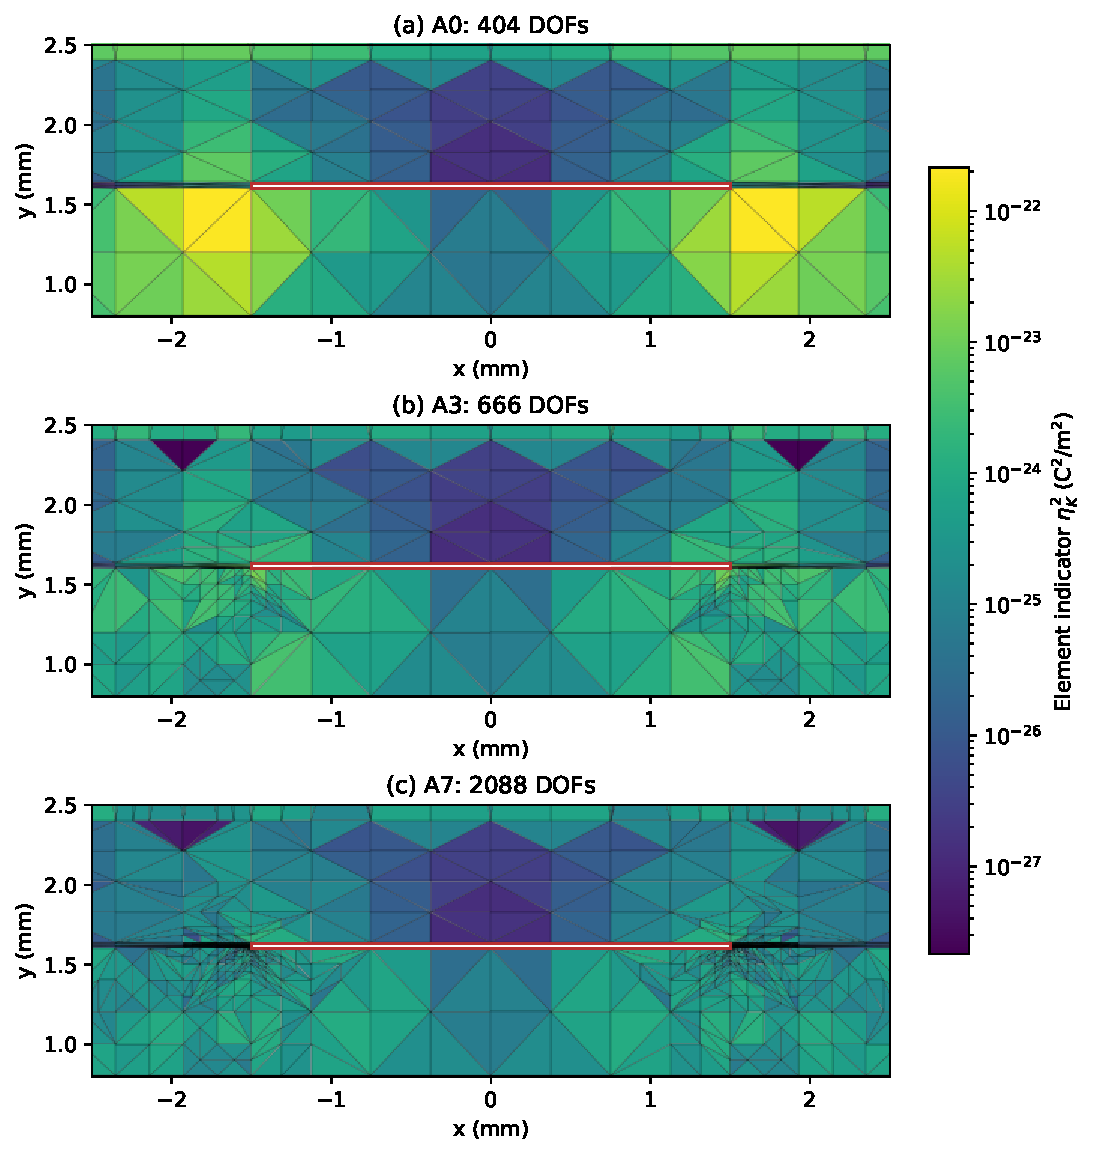
\includegraphics[width=0.88\textwidth,height=0.70\textheight,keepaspectratio]{../figures/adaptive_extension/F_ADAPTIVE_MESH_EVOLUTION.pdf}
\caption{Residual-adaptive meshes A0, A3 and A7 in the same physical near-trace window; colours show $\eta_K^2$ on a shared logarithmic scale. Refinement increasingly concentrates around the trace ends, while some marked regions lie farther into the substrate and air. This is observed localisation, not a claim that the indicator exactly identifies every singular contribution.}
\label{fig:adaptive-mesh}
\end{figure}

Within $0.25H$ of a trace corner, the element fraction rises from $5.11\%$ at A0 to $62.0\%$ at A7; these elements contain $79.6\%$ of the final squared indicator. Initially $88.6\%$ of the indicator is assigned to elements whose nearest corner is a lower junction; at A7 this fraction is $50.2\%$. Thus lower-junction concentration is strongest early, not uniformly dominant throughout. The far-boundary contribution is about $0.00265\%$ of the final indicator. Some final marked element centroids reach $|x|=5.0$ mm and $y=4.57$ mm, so refinement is not confined to four prescribed disks.

\subsection{Matched-work comparison}
One warm-up and five measured repetitions are used for every point. Uniform and graded work includes mesh generation, assembly, solve and capacitance extraction. Adaptive work is cumulative from its initial mesh, including all preceding solves, estimators, marking and refinement, up to the current solution. This accounting deliberately charges adaptive refinement for the preceding solve--estimate--mark--refine cycles because those computations are required to obtain the final adaptive mesh; the comparison is therefore conservative with respect to adaptivity. DOF and NNZ comparisons remain independent of this timing convention. Offline reference solves and error integration are excluded equally. This prevents comparing an entire adaptive trajectory with only a final sparse solve. Millisecond-scale differences on the coarsest meshes are not interpreted as convincing speedups.

\begin{figure}[H]
\centering
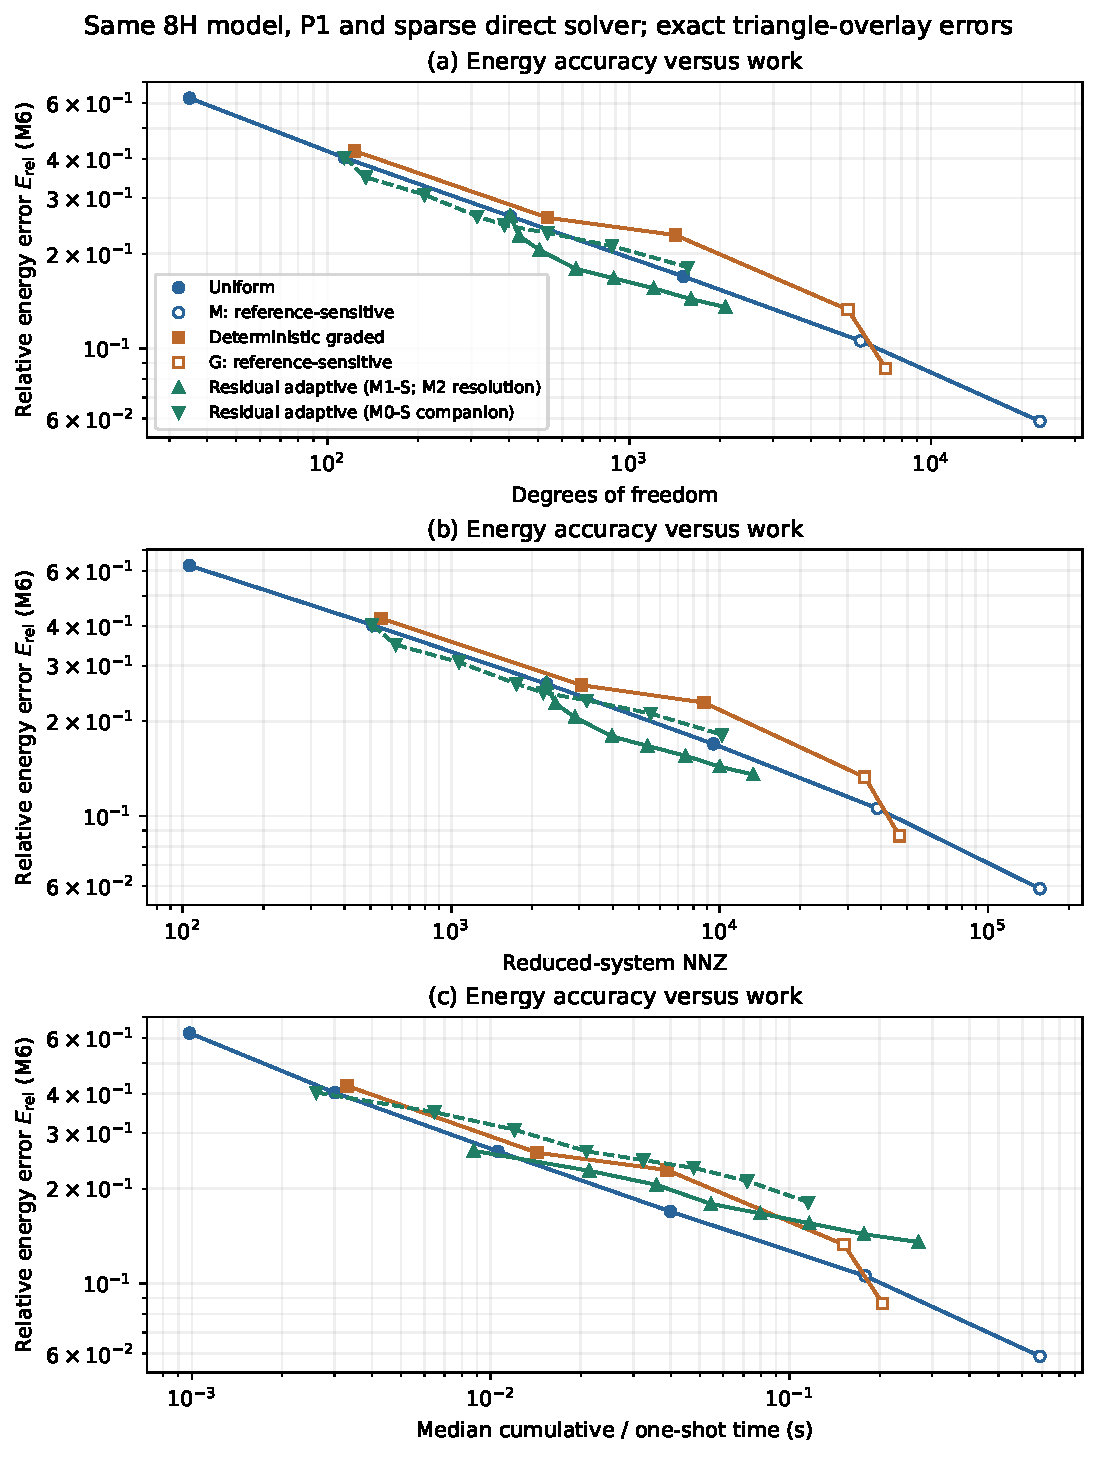
\includegraphics[width=0.92\textwidth,height=0.85\textheight,keepaspectratio]{../figures/adaptive_extension/F_ADAPTIVE_WORK_PRECISION.pdf}
\caption{New three-way comparison in a common norm: (a) DOFs, (b) reduced NNZ, (c) measured median total algorithm time. Solid green triangles are the primary M1-S path; dashed green triangles are its separately identified M0-S companion. Open markers fail the M6/M7 reference-sensitivity threshold. Historical uniform/graded raw errors and timing tables were not overwritten.}
\label{fig:adaptive-work}
\end{figure}

\begin{table}[H]
\centering\small
\caption{Piecewise log-linear interpolation between measured consecutive points only. $U,G,A$ denote uniform, prescribed grading and residual adaptivity. Ratios above one favour adaptivity. The $0.40/0.30$ adaptive targets use the M0-S companion. $^*$The $0.20$ three-way comparison is exploratory because the graded bracket includes reference-sensitive G3.}
\begin{tabular}{@{}lrrrrrr@{}}
\toprule
Target & $N_U$ & $N_G$ & $N_A$ & $N_U/N_A$ & $\mathrm{NNZ}_U/\mathrm{NNZ}_A$ & $T_U/T_A$\\
\midrule
0.40 & 116.6 & 146.2 & 115.1 & 1.013 & 1.022 & 1.115\\
0.30 & 272.8 & 348.7 & 224.0 & 1.218 & 1.235 & 0.546\\
0.20$^*$ & 917.3 & 1974.2 & 532.7 & 1.722 & 1.791 & 0.618\\
\bottomrule
\end{tabular}

\label{tab:adaptive-targets}
\end{table}

At $E_{\rm rel}=0.30$, adaptivity needs about $224$ DOFs versus $273$ for uniform and $349$ for grading, with uniform/adaptive DOF and NNZ ratios $1.218$ and $1.235$. However, its cumulative median time is $13.1$ ms versus $7.15$ ms for uniform: the time ratio is $0.546$, not a speedup. At $0.40$, the DOF ratio is only $1.013$ and the measured times are too small to establish a robust runtime advantage. In a direct reference-stable comparison, A5 uses $1206$ DOFs with error $0.1553$, while M3 uses $1512$ DOFs with error $0.1694$; A5 nevertheless takes about $2.91$ times the cumulative algorithm time.

\subsection{Interpretation and capacitance}
The extension demonstrates an approximation-size advantage at $0.30$, but not a uniform runtime advantage. A7 has $1522$ elements outside the specified corner neighbourhoods, versus $2047$ for G2 at a comparable scale. This supports the explanation that coordinate-line grading spends more resolution away from corners; it does not isolate the causal effects of band width, lower-corner weighting or transitions, which were not varied independently.

The capacitance diagnostic uses $|C_h-C_{M7}|/|C_{M7}|$, where computed M7 is a selected numerical reference, not exact capacitance. A5 differs by $2.42\%$, versus $3.03\%$ for M3, so the energy improvement also has a capacitance benefit in this matched-work pair. A7 still differs by $1.74\%$ and is not substituted for the accepted M7 engineering mesh.

\begin{figure}[H]
\centering
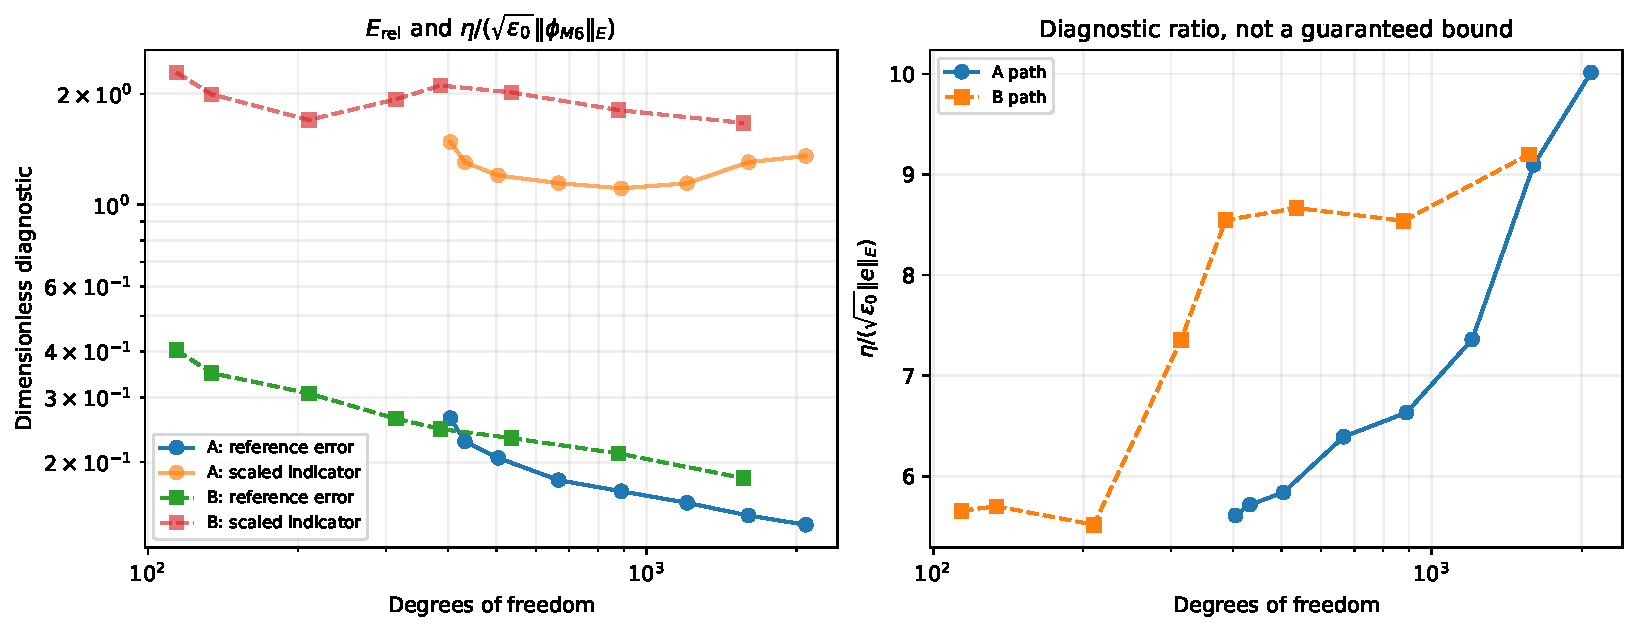
\includegraphics[width=\textwidth]{../figures/adaptive_extension/F_ADAPTIVE_ESTIMATOR.pdf}
\caption{Indicator diagnostics. Physical $\eta$ has units C/m, whereas $\|e\|_E$ has units $\sqrt{\mathrm{J/m}}$. For a dimensionless display only, $\eta$ is divided by $\sqrt{\epsilon_0}$ and the reference norm; the requested unscaled ratio $\eta/\|e\|_E$ is also stored. The dimensionless diagnostic ratio increases from about $5.61$ to $10.0$ on the primary path: it has not stabilised and is not an effectivity constant or guaranteed error bound.}
\label{fig:adaptive-estimator}
\end{figure}

The primary true reference error decreases throughout, but $\eta$ decreases initially and rises again over the last levels. Therefore this indicator is useful for selecting refinement locations in this experiment, but the data do not justify using it as a calibrated stopping criterion. All corrected A/B cycles satisfy potential bounds, symmetry, residual, matrix-symmetry, charge-balance, material and conformity checks; the failed first attempt remains explicitly archived.


\section{Final Capacitance and Effective Permittivity}
\subsection{Final dielectric capacitance}
The final capacitance selection used the nested uniform M3--M7 hierarchy on the fixed $8H$ domain. The M8 preflight indicated excessive sparse-direct factorisation cost and fill-in risk, so we did not run it. We accepted M7 through the documented resource/asymptotic fallback: capacitance decreased monotonically, and both the apparent output orders and Richardson diagnostics were stable. The final reported capacitance remains the computed M7 FEM value, not the Richardson extrapolate.
The M6--M7 change is $0.1556\%$, above the preferred $0.1\%$ target. Acceptance rests on the stated fallback criteria; the preferred target was not achieved. Write $C_k$ for the energy capacitance on uniform level M$k$. The successive relative change is $dC_k=|C_k-C_{k-1}|/|C_k|$. For approximately halved mesh sizes, the apparent output order is $p_C=\log(|C_{k-2}-C_{k-1}|/|C_{k-1}-C_k|)/\log 2$. The Richardson diagnostic is $C_{\rm ext}=C_k+(C_k-C_{k-1})/(2^{p_C}-1)$, where $C_{\rm ext}$ estimates a limiting capacitance but is not a solved FEM result. In Table~\ref{tab:richardson-robustness}, finest-to-extrapolate difference is $|C_k-C_{\rm ext}|/|C_{\rm ext}|$; limit change compares consecutive extrapolates using the newer extrapolate as denominator. The diagnostics below support this qualified acceptance while showing the remaining spatial sensitivity.
\begin{table}[H]\centering\small
\caption{Output-order and Richardson diagnostics from all available successive triples. $C_{\rm ext}$ is never substituted for the computed M7 result.}
\begin{tabular}{@{}lrrrr@{}}
\toprule
Triple & $p_C$ & $C_{\rm ext}$ (pF/m) & Finest-to-ext (\%) & Limit change (\%)\\
\midrule
M3-M4-M5 & 1.17929 & 120.487011 & 0.6127 & --\\
M4-M5-M6 & 1.15979 & 120.468826 & 0.2810 & 0.015095\\
M5-M6-M7 & 1.15524 & 120.466884 & 0.1269 & 0.001613\\
\bottomrule
\end{tabular}
\label{tab:richardson-robustness}
\end{table}


\begin{figure}[H]
\centering
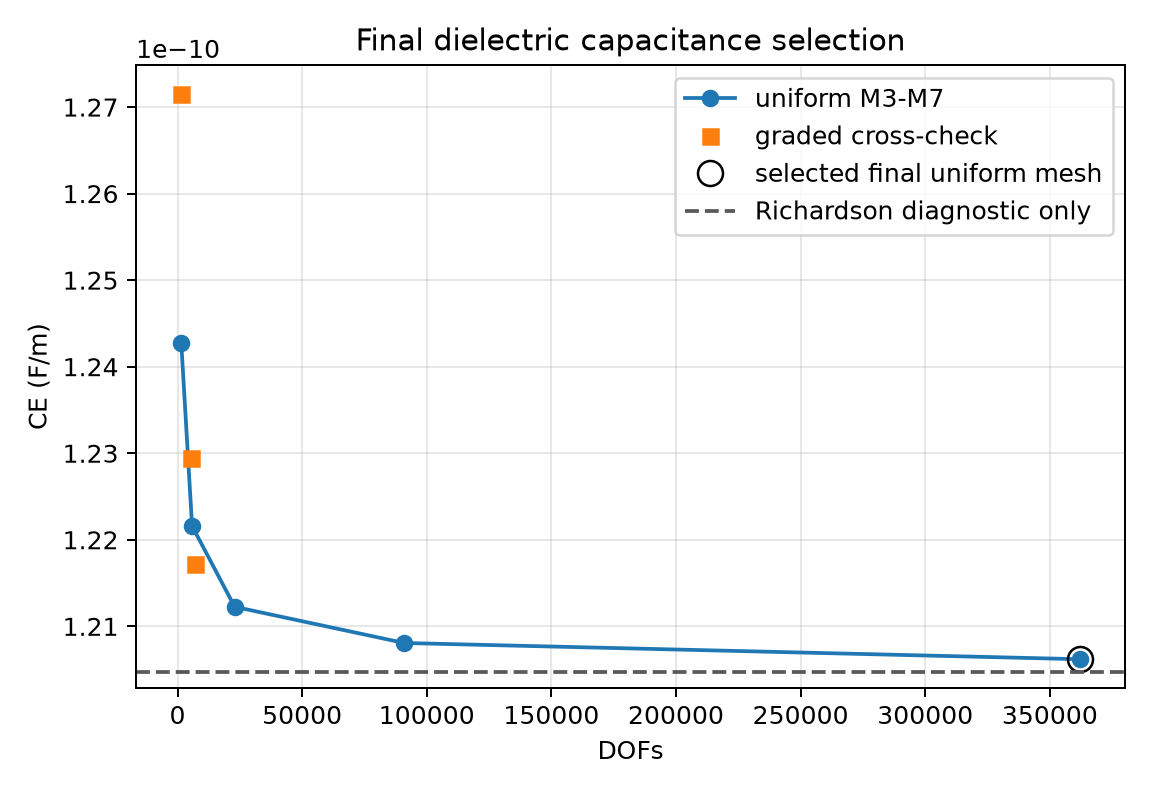
\includegraphics[width=0.82\textwidth]{final_capacitance_convergence.png}
\caption{Final dielectric capacitance selection. M7 is the selected computed FEM mesh; the Richardson line is a diagnostic only.}
\label{fig:finalcap}
\end{figure}

\begin{table}[H]
\centering
\small
\caption{Final dielectric capacitance sequence.}
\label{tab:finalcap}
\begin{tabular}{@{}rrrrr@{}}
\toprule
Mesh & Elements & DOFs & $C_E$ (pF/m) & Successive change\\
\midrule
M3 & 2816 & 1512 & 124.273 & --\\
M4 & 11264 & 5840 & 122.159 & $1.731\%$\\
M5 & 45056 & 22944 & 121.225 & $0.770\%$\\
M6 & 180224 & 90944 & 120.807 & $0.346\%$\\
M7 & 720896 & 362112 & 120.620 & $0.156\%$\\
\bottomrule
\end{tabular}
\end{table}

The M7--M6 change, $0.1556\%$, is above the preferred direct $0.1\%$ quality-control target. The reported value is the computed M7 result. Its remaining spatial sensitivity is approximately $0.156\%$, while the tested finite-domain sensitivity is approximately $0.182\%$; neither is a rigorous error bound. They are reported separately rather than combined statistically.

\subsection{Matched all-air solve and effective permittivity}
The all-air calculation reused the exact frozen M7 mesh. Only the material coefficient was changed to $\epsr=1$ everywhere. The dimensionless effective relative permittivity is $\epseff=C/\Cair$, where $C$ is the selected dielectric capacitance and $\Cair$ the capacitance with every field element assigned air permittivity. Using the same mesh keeps the material change separate from differences caused by remeshing. The mesh fingerprint, degrees of freedom, boundary sets, and matrix sparsity pattern were all checked to match.

\[
C=120.620\,\mathrm{pF/m},\qquad
\Cair=35.9682\,\mathrm{pF/m},\qquad
\epseff=\frac{C}{\Cair}=3.3535.
\]

\begin{figure}[H]
\centering
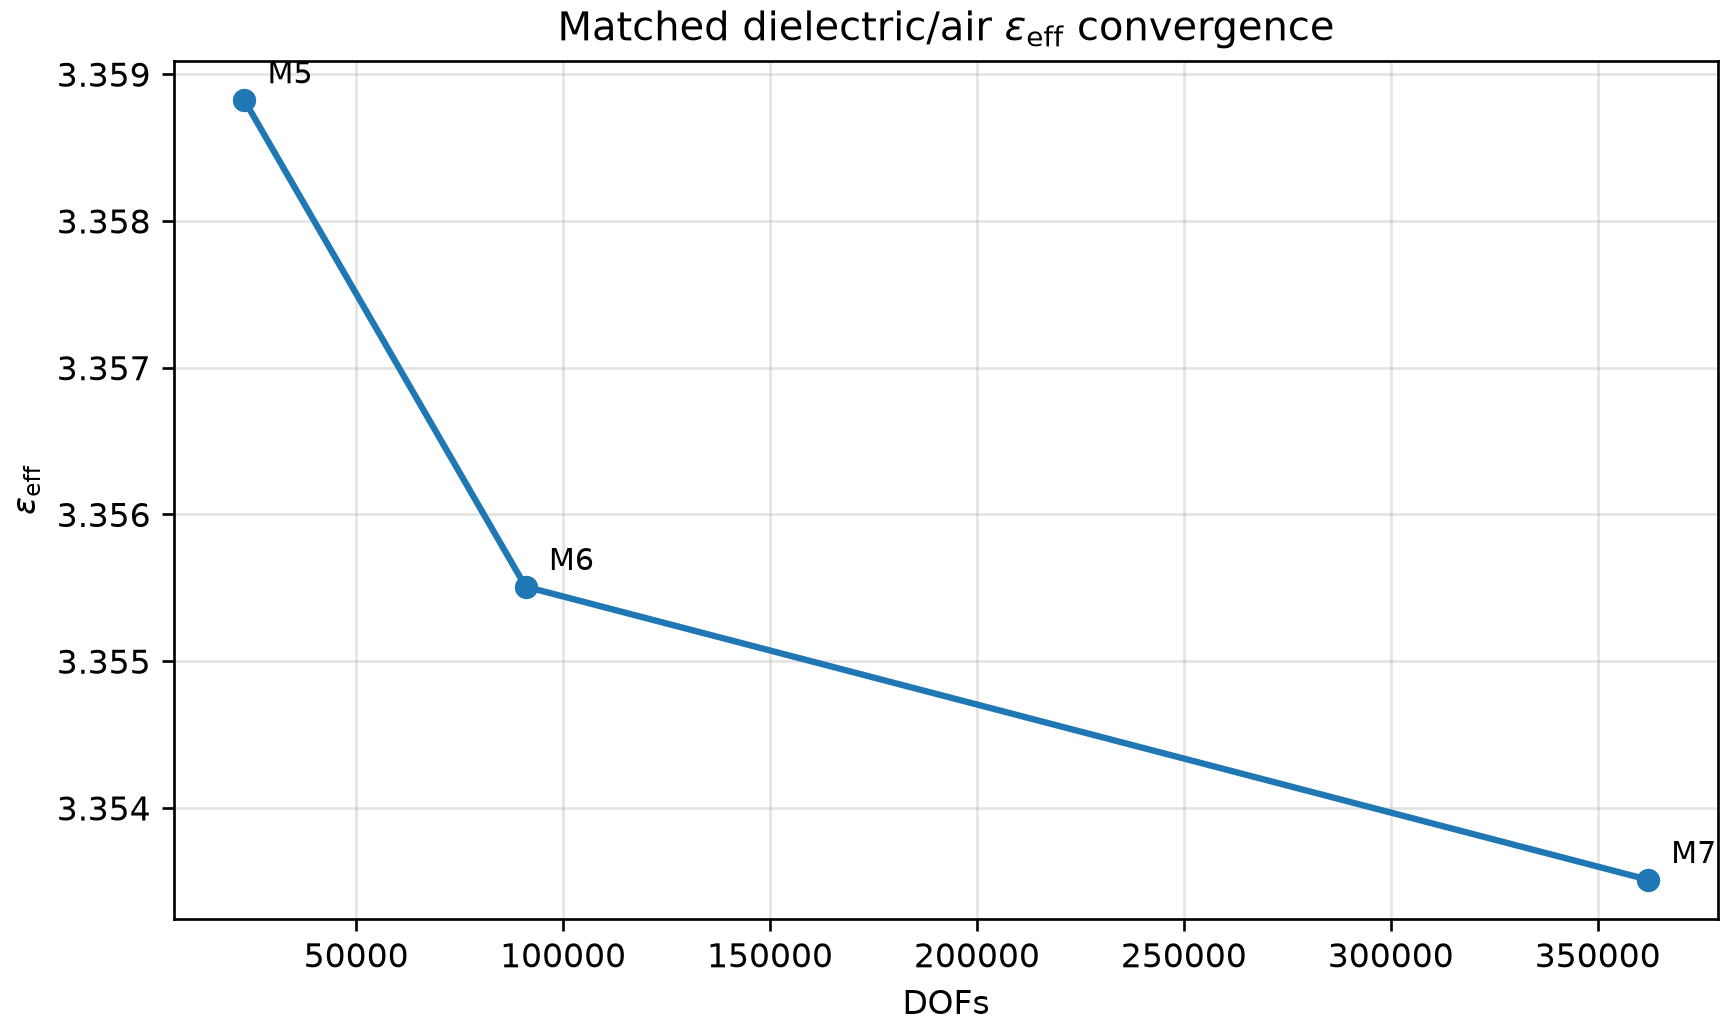
\includegraphics[width=0.82\textwidth]{epsilon_eff_convergence_report.png}
\caption{Matched M5--M7 effective-permittivity convergence. The M6--M7 relative change is about $0.0595\%$.}
\label{fig:epsconv}
\end{figure}

\section{Characteristic Impedance and Engineering Validation}
\subsection{Final quasi-TEM impedance}
Let $c_0=299792458\,\mathrm{m/s}$ be the exact SI vacuum speed of light, $L$ the quasi-TEM inductance per unit length (H/m), and $\Zzero$ the characteristic impedance ($\Omega$). Using the matched capacitance pair,
\[
L=\frac{1}{c_0^2\Cair},\qquad
\Zzero=\sqrt{\frac{L}{C}}=\frac{1}{c_0\sqrt{C\Cair}},
\]
The equivalent expression
\[
\Zzero=\frac{1}{c_0\Cair\sqrt{\epseff}}
\]
agrees to floating-point precision; this is an internal identity, not an independent validation. The phase velocity $v_p$ (m/s) is $v_p=c_0/\sqrt{\epseff}=1/\sqrt{LC}$, giving the value in Table~\ref{tab:finalengineering}.

\begin{table}[H]
\centering
\small
\caption{Final FEM transmission-line quantities.}
\label{tab:finalengineering}
\begin{tabular}{@{}ll@{}}
\toprule
Quantity & Value\\
\midrule
$C$ & $120.620\,\mathrm{pF/m}$\\
$\Cair$ & $35.9682\,\mathrm{pF/m}$\\
$\epseff$ & $3.3535$\\
$L$ & $3.09343\times10^{-7}\,\mathrm{H/m}$\\
$v_p$ & $1.63708\times10^{8}\,\mathrm{m/s}$\\
$\Zzero$ & $50.642\,\Omega$\\
\bottomrule
\end{tabular}
\end{table}

\begin{figure}[H]
\centering
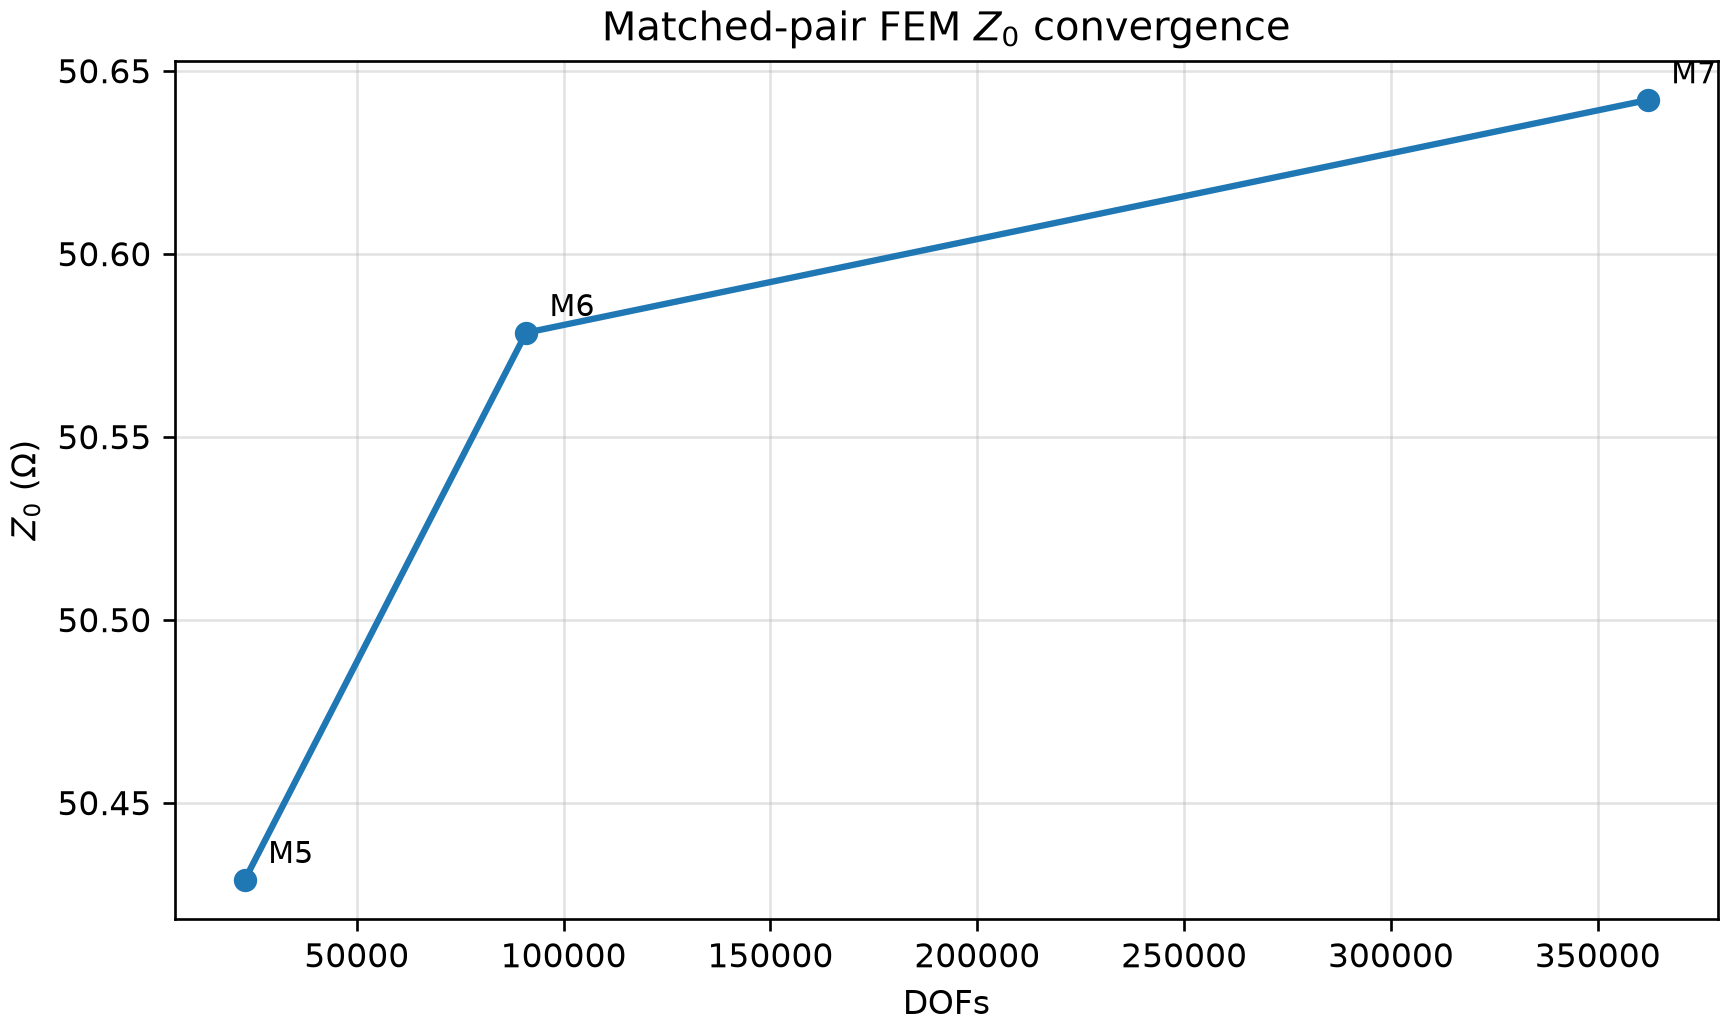
\includegraphics[width=0.82\textwidth]{Z0_convergence_report.png}
\caption{Direct matched-pair convergence of the final engineering quantity. The M6--M7 relative change in $\Zzero$ is about $0.126\%$.}
\label{fig:zconv}
\end{figure}

\subsection{Independent engineering benchmarks}
The final transmission-line table reports the computed M7 values. Their precision should be read alongside the $0.156\%$ spatial and $0.182\%$ finite-domain sensitivity indicators, rather than as exact limiting values.

The Hammerstad--Jensen and IPC-2141 calculations use only geometry and $\epsr$, not FEM capacitance or FEM $\epseff$. They are independent approximate engineering formulas, not exact solutions. The Hammerstad--Jensen implementation uses the finite strip-thickness correction from the project specification\footnote{E. Hammerstad and O. Jensen, ``Accurate Models for Microstrip Computer-Aided Design,'' \emph{1980 IEEE MTT-S International Microwave Symposium Digest}, pp.~407--409, 1980, \url{https://doi.org/10.1109/MWSYM.1980.1124303}. The specific finite-thickness variant is the one documented in the supplied \emph{Capacitor2d} appendix.}; IPC-2141 uses the compact external-microstrip expression with a natural logarithm\footnote{IPC, \emph{IPC-2141: Controlled Impedance Circuit Boards and High Speed Logic Design}, April 1996. We use the compact external-microstrip expression specified in the supplied \emph{Capacitor2d} appendix, not a new transcription of the full standard. IPC confirms the original edition on the successor cover: \url{https://www.ipc.org/TOC/IPC-2141A.pdf}.}.

Let $Z$ be any impedance being compared; $Z_{0,\rm FEM}$, $Z_{0,\rm HJ}$ and $Z_{0,\rm IPC}$ denote the FEM, Hammerstad--Jensen and IPC impedances, respectively. Following Appendix E of the specification, the dimensionless discrepancy $d_{\rm HJ}(Z)$ uses Hammerstad--Jensen in the denominator:
\[
d_{\mathrm{HJ}}(Z)=\frac{|Z-Z_{0,\mathrm{HJ}}|}{|Z_{0,\mathrm{HJ}}|}.
\]
The primary comparisons are therefore $100d_{\rm HJ}(Z_{0,\rm FEM})=0.879\%$ and $100d_{\rm HJ}(Z_{0,\rm IPC})=1.608\%$. The optional FEM-denominator differences are retained in a separately labelled column so that the two definitions cannot be confused.

\begin{figure}[H]
\centering
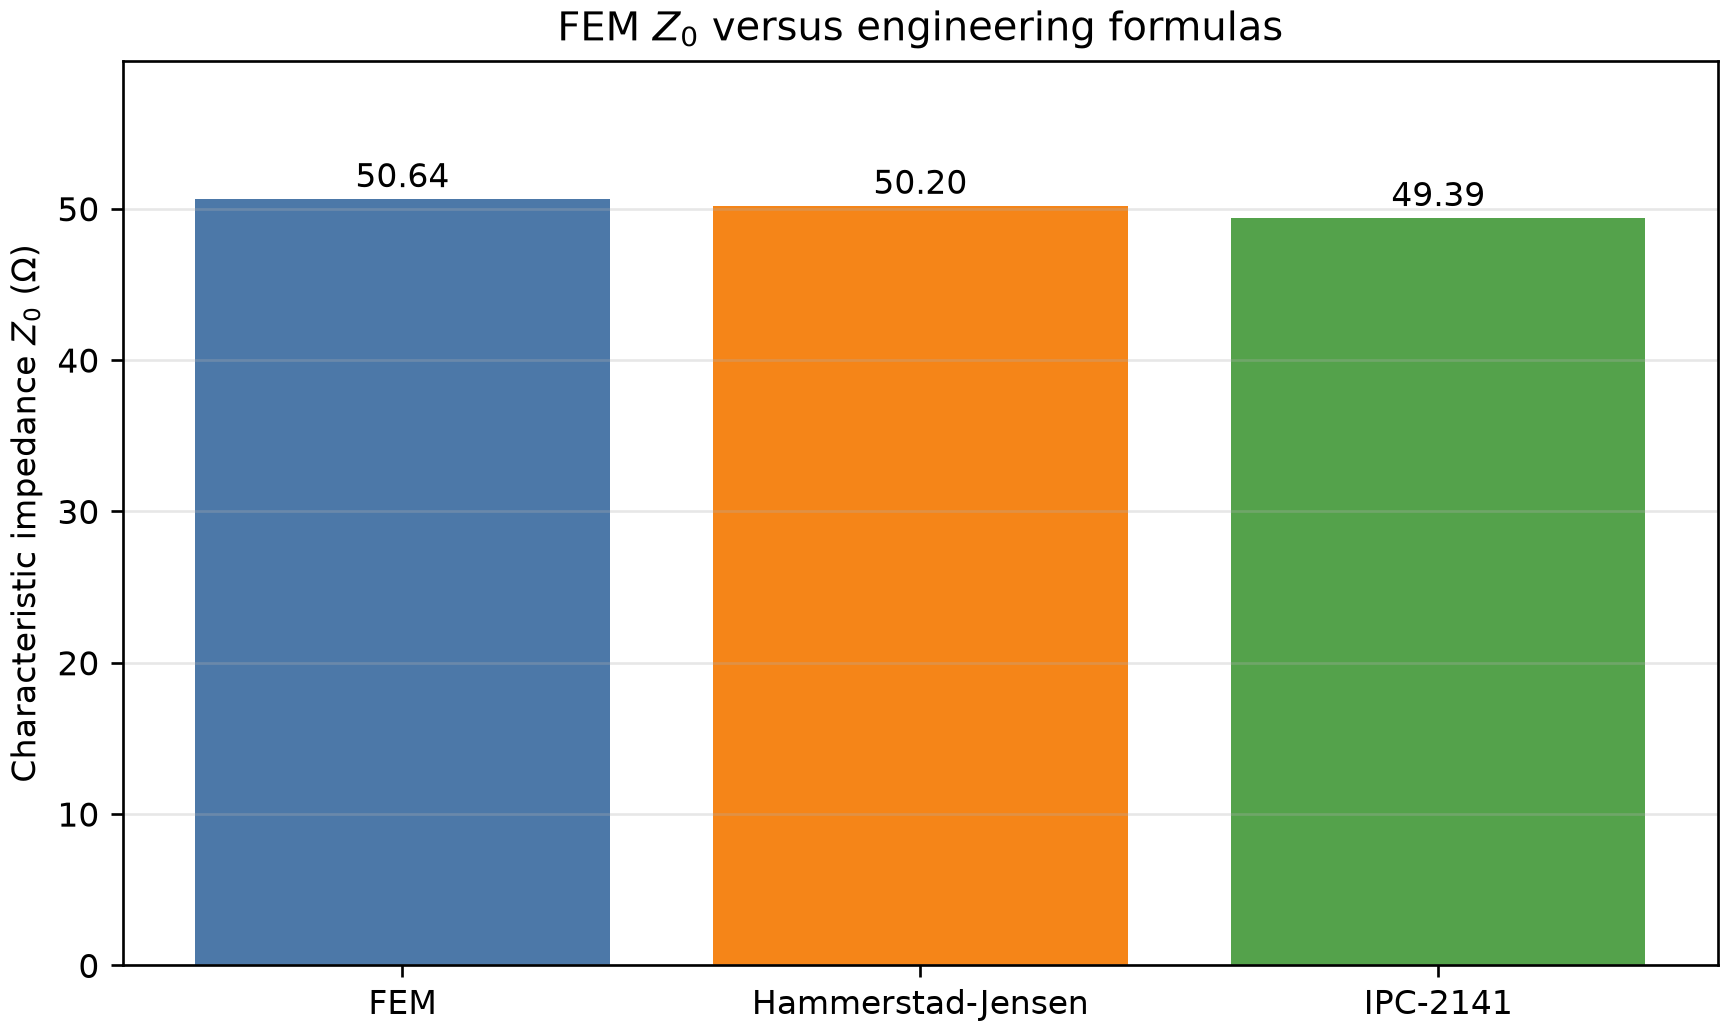
\includegraphics[width=0.82\textwidth]{Z0_benchmark_comparison_report.png}
\caption{Final FEM characteristic impedance compared with independent engineering approximations.}
\label{fig:bench}
\end{figure}

\begin{table}[H]
\centering
\small
\caption{Engineering benchmark comparison. The primary $d_{\rm HJ}$ column uses the specification's Hammerstad--Jensen denominator. The last column is the supplementary $|Z-Z_{0,\rm FEM}|/|Z_{0,\rm FEM}|$ percentage, not $d_{\rm HJ}$.}
\label{tab:bench}
\begin{tabular}{@{}lrrrr@{}}
\toprule
Method & $\varepsilon_{\rm eff}$ & $Z_0$ ($\Omega$) & $100d_{\rm HJ}$ & Diff. vs FEM\\
\midrule
FEM matched pair & 3.3535 & 50.642 & $0.879\%$ & $0.000\%$\\
Hammerstad--Jensen & 3.3008 & 50.201 & $0.000\%$ & $0.871\%$\\
IPC-2141 & -- & 49.393 & $1.608\%$ & $2.466\%$\\
\bottomrule
\end{tabular}

\end{table}

The Hammerstad--Jensen formula agrees more closely with the FEM result than the simpler IPC-2141 expression. The agreement supports the scale of the engineering result. Its numerical reliability rests primarily on the verification and convergence studies, since agreement with an approximation cannot prove FEM correctness.

The final FEM value is also close to the common $50\,\Omega$ design target:
\[
\Zzero-50\,\Omega = 0.642\,\Omega,
\]
or about $1.284\%$ above $50\,\Omega$. The target is design context only, not a numerical reference solution.

\section{Limitations}
The physical model is electrostatic and quasistatic/quasi-TEM. It does not include dielectric dispersion, dielectric loss, conductor loss, surface roughness, solder-mask loading, radiation, anisotropy, or manufacturing tolerances. The trace and ground are perfect conductors.

Several numerical limitations remain. The $8H$ domain is justified by a finite $12H$ comparison, not by an exact infinite-domain solution. The final M7 mesh was accepted through a resource-aware asymptotic fallback rather than by directly reaching the preferred $0.1\%$ capacitance-change target. Richardson extrapolation is diagnostic only. The historical graded curves use approximate cross-mesh quadrature; only the separately recomputed exact-overlay extension is used for current quantitative efficiency claims. The adaptive comparison uses one residual indicator, a primary D\"orfler parameter ($\theta=0.5$) with a separate $0.3/0.7$ sensitivity study, one symmetry/conformity closure and two declared starting meshes. It does not establish optimality among estimators or marking strategies; the indicator-to-error ratio has not stabilised.

\subsection*{Reproduction commands and current scope}
The pinned environment uses Python 3.13.13, NumPy 2.5.2, SciPy 1.18.1, Matplotlib 3.11.1, scikit-fem 12.0.2, Shapely 2.1.2 and pytest 9.1.1. The recorded machine is an Apple M2 with 16 GB RAM running macOS 26.6.2. Install the combined requirements and run from the repository root:
\begin{verbatim}
python3 -m pip install -r requirements-adaptive.txt
pytest -q
python3 code/run_all.py --quick
python3 code/run_all.py --full
\end{verbatim}
Quick mode checks saved evidence and rebuilds plots in an isolated directory; it does not recompute the final M7 quantities. Full mode starts from numerical solves, replays the frozen mesh, and runs the overlay/adaptive comparison. It backs up the existing evidence and compares fresh output against it rather than overwriting it. The invalid graded shortcut still rejects crossed triangles; the integrated route explicitly selects polygon-overlay integration instead.

The first integrated run completed in about 190 s on this machine, passing 208 numerical comparisons with unchanged original protected files and the same final-mesh fingerprint. A later final-code run and its exact commands, resource preflight, tests and output manifests are recorded under \path{reproduction/} and \path{logs/ae_reproduction_report.md}. Regression testing currently reports 58 passed with no skips. These runs verify the pinned local environment. A clean installation on a different operating system has not been tested. M8 is intentionally excluded. Timings vary: at the $0.30$ target the first rerun gave adaptive/uniform cumulative time about $1.90$, compared with $1.83$ in the original experiment, preserving the qualitative runtime conclusion.

\section{Conclusions}
For the studied microstrip geometry, the selected M7 solution gives $C=120.620\,\mathrm{pF/m}$. The all-air solve on exactly the same mesh gives $\Cair=35.9682\,\mathrm{pF/m}$, leading to $\epseff=3.3535$ and $\Zzero=50.642\,\Omega$. This is close to the common $50\,\Omega$ design target.

At relative energy error $0.30$, residual-based adaptivity needs approximately $224$ DOFs, compared with $273$ for uniform refinement and $349$ for grading. It uses fewer DOFs and matrix nonzeros, but its cumulative time is $13.1$ ms compared with $7.15$ ms for uniform refinement. The repeated solve--estimate--mark--refine cycles account for this extra work. At the tested target, reducing the number of unknowns did not reduce total runtime.

The M6--M7 spatial indicator is approximately $0.156\%$, while the separate, coarser matched-core domain study gives $0.182\%$. Neither is a rigorous error bound, and the latter is not a measured M7 truncation error. M7 was accepted through the documented resource/asymptotic fallback, and Richardson extrapolation remains diagnostic. The quasi-static model also omits losses and full-wave dispersion or radiation, so the reported impedance should be interpreted within those assumptions.


\bibliographystyle{plain}
\bibliography{references}

\appendix
\section{AI Transparency Audit}
We used AI/Codex for code scaffolding, plotting, workflow generation, documentation, consistency checks and report drafting and revision. We checked the numerical claims with manufactured solutions, matrix and residual diagnostics, domain and refinement studies, matched-mesh replay and independent formulas. The first three cases below record assumptions, possible falsifiers, evidence locations and decisions; the last two cover additional checks. These checks concern the numerical claims and do not by themselves establish individual authorship or complete pipeline certification.

The audit also follows the five-gate process required for AI-assisted solver work. First, formula and equation transcription was checked against the project source documents. Second, structure and indexing risks were tested through geometry, material-region, boundary-node, and dof checks. Third, the mathematical formulation was checked by deriving the weak form, Dirichlet elimination, capacitance identities, and quasi-TEM identities explicitly. Fourth, independent reproduction was addressed by the manufactured-solution test, mesh-refinement studies, matched air-only replay, and engineering benchmark formulas. Fifth, suspicious or fragile results were interrogated through the dedicated domain, reference-stability, graded-refinement, final-capacitance, and matched-mesh studies rather than accepted at face value.

\begin{longtable}{@{}L{0.22\textwidth}L{0.32\textwidth}L{0.36\textwidth}@{}}
\caption{Project-specific AI audit summary.}\label{tab:aiaudit}\\
\toprule
Component & Main risk & Verification evidence\\
\midrule
\endfirsthead
\toprule
Component & Main risk & Verification evidence\\
\midrule
\endhead
P1 FEM solver and Dirichlet elimination & Incorrect assembly, boundary treatment, or material coefficient handling & Manufactured-solution convergence; matrix symmetry and residual checks; material-tag tests\\
Microstrip geometry & Trace hole, interface, or boundary nodes misidentified & Geometry tests; full and near-trace figures; potential bounds and symmetry\\
Capacitance extraction & Reaction sign or trace-dof summation error & $C_E/C_Q$ agreement and charge-balance diagnostics\\
Domain study & Changing the far domain could also change the near-trace mesh & Automated near-field equivalence checks and domain-truncation tables\\
Uniform convergence & Invalid coefficient-vector subtraction across meshes & Reference-mesh gradient transfer and reference-stability table\\
Graded refinement & Confusing coordinate nesting with triangular common refinement & Geometry audit detects crossed diagonals; original efficiency estimates retained with an explicit integration caveat\\
Final capacitance & Selecting a convenient mesh rather than an evidenced one & M3--M7 monotonic sequence, M8 preflight, Richardson diagnostic, frozen mesh artifact\\
Matched all-air solve & Regenerating a nominally similar mesh and contaminating $C/\Cair$ & Frozen mesh SHA-256, same dofs, same boundary sets, same sparse pattern, dielectric replay\\
Engineering benchmarks & Circular validation using FEM outputs inside formulas & Benchmark function signatures accept only geometry and $\epsr$; unit-invariance tests\\
\bottomrule
\end{longtable}

\paragraph{Case audit 1: energy--charge agreement.}

\noindent\textit{Claim examined:} near-equality of $C_E$ and $C_Q$ proves spatial convergence.

\noindent\textit{Assumptions:} both quantities use the same discrete potential, stiffness operator, prescribed voltage and material-conforming element integrals.

\noindent\textit{Risk and falsifier:} reactions and energy come from the same stiffness matrix, so even a coarse mesh can satisfy $2W_e=V_0Q_{\rm trace}$.

\noindent\textit{Independent evidence:} M0 has $\delta_{EQ}\approx4.62\times10^{-16}$ but $C_E\approx167.703\,\mathrm{pF/m}$, whereas the computed M7 result is $120.620\,\mathrm{pF/m}$.

\noindent\textit{Evidence locations:} \path{tables/uniform_convergence.csv} (M0), \path{tables/final_capacitance_convergence.csv} (M3--M7), and \path{logs/gate_F_capacitance.txt}; the extraction is \texttt{extract\_capacitance} in \path{code/capacitance.py}, with regression checks in \path{code/tests/test_final_capacitance.py}. The refinement sequence tests the convergence claim independently of the shared matrix identity.

\noindent\textit{Decision:} reject that inference; use $\delta_{EQ}$ for algebraic consistency and the separate mesh sequence for spatial sensitivity.

\noindent\textit{Remaining limitation:} the mesh sequence still has the disclosed M7 fallback sensitivity.

\paragraph{Case audit 2: a finite far-boundary reference.}

\noindent\textit{Claim examined:} the tested $12H$ solution is the exact infinite-domain answer.

\noindent\textit{Assumptions:} all four domains retain homogeneous Neumann outer boundaries and the same near-field mesh; only the outer region is extended.

\noindent\textit{Risk and falsifier:} a finite Neumann boundary still changes the field; one large box alone cannot remove truncation.

\noindent\textit{Independent evidence:} the fixed-core 3H--12H sequence and the finer 12H repeat separate measured domain and mesh effects.

\noindent\textit{Evidence locations:} \path{tables/domain_truncation.csv}, \path{tables/domain_mesh_adequacy.csv} and \path{logs/gate_C_domain.txt}; generation is in \path{code/domain_study.py}, and fixed-core/domain checks are in \path{code/tests/test_domain_study.py}. Figure~\ref{fig:domain} displays the production comparison; Table~\ref{tab:domain} and its following paragraph report the fine-domain check.

\noindent\textit{Decision:} call 12H a tested finite-domain reference and report the $0.182\%$ 8H difference separately.

\noindent\textit{Remaining limitation:} no exact infinite-domain error bound is available. The case examines that inference; it does not claim that the project previously presented an exact infinite-domain reference.

\newpage
\paragraph{Case audit 3: errors across different meshes.}

\noindent\textit{Claim examined:} coefficient vectors or nested coordinate lists alone define a valid cross-mesh energy error.

\noindent\textit{Assumptions:} the original shortcut treated every reference triangle as lying within one coarse triangle, so both gradients were constant on the integration cell.

\noindent\textit{Risk and falsifier:} vector entries live in different bases, and a fine triangle crossing a coarse gradient jump invalidates constant-gradient element integration.

\noindent\textit{Independent evidence:} uniform triangle-containment checks pass, while the new vertex-side test finds crossings in all five graded cases despite coordinate-subset tests passing.

\noindent\textit{Decision at the rubric review:} retain the uniform norm calculation, correct the graded guard, and withdraw precise graded efficiency claims until overlay integration is validated.

\noindent\textit{Extension verification:} Section~\ref{sec:residual-adaptive} subsequently supplies separately stored exact-overlay errors for all three methods. Opposite-diagonal analytic integration, the nested Galerkin identity, material matching and area-coverage tests support that implementation. Historical curves were not overwritten.

\begin{sloppypar}
\noindent\textit{Evidence locations:} \path{tables/graded_reference_geometry_audit.csv} records crossings; \texttt{common\_refinement\_diagnostics} in \path{code/graded_study.py} checks them. The replacement integration is \texttt{overlay\_energy\_error} in \path{code/overlay_energy.py}. Its independent tests are \path{test_exact_overlay_crossing_diagonals} and \path{test_overlay_reproduces_uniform_nested_energy_identity} in \path{code/tests/test_residual_adaptive.py}. Current errors and formal targets are in \path{results/adaptive_extension/uniform_graded_overlay_comparison.csv} and \path{results/adaptive_extension/adaptive_matched_targets.csv}; \path{logs/adaptive_final_validation.txt} records the standalone run validation.
\end{sloppypar}

\noindent\textit{Remaining limitation:} fine graded points remain reference-sensitive. The revised unified entry now uses overlays and has been rerun; the historical centroid shortcut remains blocked. Cross-platform reproduction remains untested.

\paragraph{Case audit 4: symmetry and mesh-quality assumptions.}

\noindent\textit{Claim examined:} symmetric node coordinates alone ensure a symmetric continuous $P_1$ field after local refinement.

\noindent\textit{Falsifier and evidence:} historical parallel diagonals gave an approximately $2.05\%$ continuous reflection discrepancy on M2 despite near-roundoff nodal symmetry. A first diagonal-only completion then failed coarse-companion potential bounds.

\noindent\textit{Decision:} retain the failed attempt, use a nonobtuse mirror completion of the same parent family, and test continuous reflection, bounds, conformity and material tags independently. The corrected paths pass these checks; $\theta$ was not tuned to obtain a favourable efficiency result.

\paragraph{Additional coefficient and reproduction checks.}
The layered analytic test uses the production assembly, while its unresolved-interface control shows that small residuals and an SPD matrix can coexist with a wrong material model. Evidence is in \path{code/layered_verification.py}, \path{code/tests/test_layered_verification.py} and \path{results/ae_revision/layered_interface_verification.csv}. The renewed reproduction is checked by \path{code/reproduction.py} and \path{code/tests/test_reproduction.py}; a failed command or changed frozen value is an error, not a successful run. Raw numerical comparisons and resource decisions are retained under \path{reproduction/}. No Git development history was manufactured; the available history remains dominated by upload commits.

\paragraph{Case audit 5: estimator interpretation.}

\noindent\textit{Claim examined:} a residual indicator is automatically a calibrated true-error estimate.

\noindent\textit{Falsifier and evidence:} the primary reference error decreases, while the final indicator rises and the scaled indicator/error ratio changes from about $5.61$ to $10.0$.

\noindent\textit{Decision:} use $\eta$ for marking only; report its dimensional and scaled diagnostics without a guaranteed-bound or stable-effectivity claim. Efficiency claims use independently integrated reference errors, not $\eta$.

\clearpage
\section{Individual Contribution Statements}

\begin{description}[style=nextline,leftmargin=0pt,labelwidth=0pt]
\item[Member 1:] \textbf{Chuqiao Tang (2360692)}. \todo{TO BE COMPLETED BY TEAM.}
\item[Member 2:] \textbf{Jinyu Ma (2363433)}. \todo{TO BE COMPLETED BY TEAM.}
\item[Member 3:] \textbf{Muqing Xu (2362900)}.

\item[Member 4:] \textbf{Shuoran Fu (2362626)}.

I worked on developing and organising the Python FEM code, including mesh generation, boundary conditions, sparse matrix assembly and solution of the electrostatic problem. My work covered files such as \path{code/geometry.py}, \path{code/fem_solver.py} and \path{code/run_all.py}. I also worked on numerical experiments involving domain size, mesh refinement, convergence analysis and adaptive refinement. I examined the results to identify numerical issues and improve the reliability of the implementation.

For the report, I designed the overall structure and contributed to writing and revising the technical sections in \path{report/main.tex}. These sections explain the mathematical model, FEM method, verification process, numerical experiments and conclusions. I organised figures and tables, checked numerical values, and revised the discussion to reflect the limitations identified during testing.

AI tools assisted with coding, debugging and writing. I reviewed the generated content and checked important results against the mathematical model and numerical evidence. My main contribution was connecting the implementation, numerical experiments and report into a consistent project.

\noindent\textit{Repository evidence:} commits \texttt{2b9dfed} and \texttt{b5eee20} record the code and report uploads under Shuoran Fu's account; \texttt{7119103} records the frozen M7 mesh addition. These are delivery records supporting the supplied statement, not a complete record of individual development steps.

\item[Member 5:] \textbf{Taiqi Zhang (2363684)}. \todo{TO BE COMPLETED BY TEAM.}
\item[Member 6:] \textbf{Yujia Ding (2362094)}.
\end{description}

\end{document}
